\documentclass[twoside]{book}

% Packages required by doxygen
\usepackage{calc}
\usepackage{doxygen}
\usepackage{graphicx}
\usepackage[utf8]{inputenc}
\usepackage{makeidx}
\usepackage{multicol}
\usepackage{multirow}
\usepackage{textcomp}
\usepackage[table]{xcolor}

% Font selection
\usepackage[T1]{fontenc}
\usepackage{mathptmx}
\usepackage[scaled=.90]{helvet}
\usepackage{courier}
\usepackage{amssymb}
\usepackage{sectsty}
\renewcommand{\familydefault}{\sfdefault}
\allsectionsfont{%
  \fontseries{bc}\selectfont%
  \color{darkgray}%
}
\renewcommand{\DoxyLabelFont}{%
  \fontseries{bc}\selectfont%
  \color{darkgray}%
}

% Page & text layout
\usepackage{geometry}
\geometry{%
  a4paper,%
  top=2.5cm,%
  bottom=2.5cm,%
  left=2.5cm,%
  right=2.5cm%
}
\tolerance=750
\hfuzz=15pt
\hbadness=750
\setlength{\emergencystretch}{15pt}
\setlength{\parindent}{0cm}
\setlength{\parskip}{0.2cm}
\makeatletter
\renewcommand{\paragraph}{%
  \@startsection{paragraph}{4}{0ex}{-1.0ex}{1.0ex}{%
    \normalfont\normalsize\bfseries\SS@parafont%
  }%
}
\renewcommand{\subparagraph}{%
  \@startsection{subparagraph}{5}{0ex}{-1.0ex}{1.0ex}{%
    \normalfont\normalsize\bfseries\SS@subparafont%
  }%
}
\makeatother

% Headers & footers
\usepackage{fancyhdr}
\pagestyle{fancyplain}
\fancyhead[LE]{\fancyplain{}{\bfseries\thepage}}
\fancyhead[CE]{\fancyplain{}{}}
\fancyhead[RE]{\fancyplain{}{\bfseries\leftmark}}
\fancyhead[LO]{\fancyplain{}{\bfseries\rightmark}}
\fancyhead[CO]{\fancyplain{}{}}
\fancyhead[RO]{\fancyplain{}{\bfseries\thepage}}
\fancyfoot[LE]{\fancyplain{}{}}
\fancyfoot[CE]{\fancyplain{}{}}
\fancyfoot[RE]{\fancyplain{}{\bfseries\scriptsize Generated on Wed Nov 29 2017 02\-:30\-:20 for Champ\-Net by Doxygen }}
\fancyfoot[LO]{\fancyplain{}{\bfseries\scriptsize Generated on Wed Nov 29 2017 02\-:30\-:20 for Champ\-Net by Doxygen }}
\fancyfoot[CO]{\fancyplain{}{}}
\fancyfoot[RO]{\fancyplain{}{}}
\renewcommand{\footrulewidth}{0.4pt}
\renewcommand{\chaptermark}[1]{%
  \markboth{#1}{}%
}
\renewcommand{\sectionmark}[1]{%
  \markright{\thesection\ #1}%
}

% Indices & bibliography
\usepackage{natbib}
\usepackage[titles]{tocloft}
\setcounter{tocdepth}{3}
\setcounter{secnumdepth}{5}
\makeindex

% Hyperlinks (required, but should be loaded last)
\usepackage{ifpdf}
\ifpdf
  \usepackage[pdftex,pagebackref=true]{hyperref}
\else
  \usepackage[ps2pdf,pagebackref=true]{hyperref}
\fi
\hypersetup{%
  colorlinks=true,%
  linkcolor=blue,%
  citecolor=blue,%
  unicode%
}

% Custom commands
\newcommand{\clearemptydoublepage}{%
  \newpage{\pagestyle{empty}\cleardoublepage}%
}


%===== C O N T E N T S =====

\begin{document}

% Titlepage & ToC
\hypersetup{pageanchor=false}
\pagenumbering{roman}
\begin{titlepage}
\vspace*{7cm}
\begin{center}%
{\Large Champ\-Net \\[1ex]\large 0.\-0.\-1 }\\
\vspace*{1cm}
{\large Generated by Doxygen 1.8.6}\\
\vspace*{0.5cm}
{\small Wed Nov 29 2017 02:30:20}\\
\end{center}
\end{titlepage}
\clearemptydoublepage
\tableofcontents
\clearemptydoublepage
\pagenumbering{arabic}
\hypersetup{pageanchor=true}

%--- Begin generated contents ---
\chapter{Hierarchical Index}
\section{Class Hierarchy}
This inheritance list is sorted roughly, but not completely, alphabetically\-:\begin{DoxyCompactList}
\item Attribute\begin{DoxyCompactList}
\item \contentsline{section}{Bit\-Serialize\-Attribute}{\pageref{class_bit_serialize_attribute}}{}
\end{DoxyCompactList}
\item Editor\begin{DoxyCompactList}
\item \contentsline{section}{Attack\-Object\-Editor}{\pageref{class_attack_object_editor}}{}
\item \contentsline{section}{Game\-State\-Editor}{\pageref{class_game_state_editor}}{}
\end{DoxyCompactList}
\item Event\-Network\begin{DoxyCompactList}
\item \contentsline{section}{Event\-Client\-Joined}{\pageref{class_event_client_joined}}{}
\item \contentsline{section}{Event\-Connected}{\pageref{class_event_connected}}{}
\item \contentsline{section}{Event\-Connection\-Rejected}{\pageref{class_event_connection_rejected}}{}
\item \contentsline{section}{Event\-Disconnected}{\pageref{class_event_disconnected}}{}
\item \contentsline{section}{Event\-Game\-State}{\pageref{class_event_game_state}}{}
\item \contentsline{section}{Event\-With\-I\-D}{\pageref{class_event_with_i_d}}{}
\begin{DoxyCompactList}
\item \contentsline{section}{Event\-Client\-Left}{\pageref{class_event_client_left}}{}
\item \contentsline{section}{Event\-With\-Player\-I\-D}{\pageref{class_event_with_player_i_d}}{}
\begin{DoxyCompactList}
\item \contentsline{section}{Event\-Request\-Player}{\pageref{class_event_request_player}}{}
\item \contentsline{section}{Event\-With\-Location}{\pageref{class_event_with_location}}{}
\begin{DoxyCompactList}
\item \contentsline{section}{Event\-Request\-Movement}{\pageref{class_event_request_movement}}{}
\end{DoxyCompactList}
\item \contentsline{section}{Event\-With\-Rank}{\pageref{class_event_with_rank}}{}
\begin{DoxyCompactList}
\item \contentsline{section}{Event\-Send\-Rank}{\pageref{class_event_send_rank}}{}
\end{DoxyCompactList}
\item \contentsline{section}{Event\-With\-Score}{\pageref{class_event_with_score}}{}
\begin{DoxyCompactList}
\item \contentsline{section}{Event\-Increment\-Score}{\pageref{class_event_increment_score}}{}
\end{DoxyCompactList}
\end{DoxyCompactList}
\end{DoxyCompactList}
\end{DoxyCompactList}
\item \contentsline{section}{Game}{\pageref{class_game}}{}
\item \contentsline{section}{I\-Serializing}{\pageref{interface_i_serializing}}{}
\begin{DoxyCompactList}
\item \contentsline{section}{Game\-State}{\pageref{class_game_state}}{}
\item \contentsline{section}{Game\-State.\-Player}{\pageref{struct_game_state_1_1_player}}{}
\end{DoxyCompactList}
\item Mono\-Behaviour\begin{DoxyCompactList}
\item \contentsline{section}{Battle\-Handler}{\pageref{class_battle_handler}}{}
\item \contentsline{section}{Bit\-Test}{\pageref{class_bit_test}}{}
\item \contentsline{section}{Camera\-Blit}{\pageref{class_camera_blit}}{}
\item \contentsline{section}{Camera\-Controller}{\pageref{class_camera_controller}}{}
\item \contentsline{section}{Camera\-Pixel\-Corrector}{\pageref{class_camera_pixel_corrector}}{}
\item \contentsline{section}{Keeper\-System}{\pageref{class_keeper_system}}{}
\item \contentsline{section}{Manager\-Transitions}{\pageref{class_manager_transitions}}{}
\item \contentsline{section}{Minimap\-Handler}{\pageref{class_minimap_handler}}{}
\item \contentsline{section}{Player\-Character\-Controller}{\pageref{class_player_character_controller}}{}
\item \contentsline{section}{Player\-Input\-Controller}{\pageref{class_player_input_controller}}{}
\item \contentsline{section}{Player\-Reference}{\pageref{class_player_reference}}{}
\begin{DoxyCompactList}
\item \contentsline{section}{Player\-Local}{\pageref{class_player_local}}{}
\begin{DoxyCompactList}
\item \contentsline{section}{Player\-Local\-Multiplayer}{\pageref{class_player_local_multiplayer}}{}
\end{DoxyCompactList}
\item \contentsline{section}{Player\-Network}{\pageref{class_player_network}}{}
\end{DoxyCompactList}
\item \contentsline{section}{Scene\-Transition}{\pageref{class_scene_transition}}{}
\item \contentsline{section}{Score\-Board}{\pageref{class_score_board}}{}
\item \contentsline{section}{Scoreboard\-Increment\-Test}{\pageref{class_scoreboard_increment_test}}{}
\item \contentsline{section}{Singleton$<$ T $>$}{\pageref{class_singleton_3_01_t_01_4}}{}
\begin{DoxyCompactList}
\item \contentsline{section}{Game\-Manager}{\pageref{class_game_manager}}{}
\item \contentsline{section}{Net\-Interface}{\pageref{class_net_interface}}{}
\end{DoxyCompactList}
\item \contentsline{section}{Transition\-Shader}{\pageref{class_transition_shader}}{}
\begin{DoxyCompactList}
\item \contentsline{section}{Transition}{\pageref{class_transition}}{}
\end{DoxyCompactList}
\item \contentsline{section}{U\-I\-Input}{\pageref{class_u_i_input}}{}
\end{DoxyCompactList}
\item \contentsline{section}{Monster\-Data\-Object}{\pageref{class_monster_data_object}}{}
\item \contentsline{section}{Champ\-Net\-Plugin.\-Network}{\pageref{class_champ_net_plugin_1_1_network}}{}
\item \contentsline{section}{Champ\-Net\-:\-:Network}{\pageref{class_champ_net_1_1_network}}{}
\item \contentsline{section}{Champ\-Net\-:\-:Packet}{\pageref{class_champ_net_1_1_packet}}{}
\item \contentsline{section}{Packet\-Battle\-Response}{\pageref{struct_packet_battle_response}}{}
\item \contentsline{section}{Packet\-Client\-Player\-I\-D}{\pageref{struct_packet_client_player_i_d}}{}
\item \contentsline{section}{Packet\-General}{\pageref{struct_packet_general}}{}
\item \contentsline{section}{Packet\-Player\-Position}{\pageref{struct_packet_player_position}}{}
\item \contentsline{section}{Packet\-Player\-Scoreboard\-Info}{\pageref{struct_packet_player_scoreboard_info}}{}
\item \contentsline{section}{Champ\-Net\-:\-:Packet\-Queue}{\pageref{class_champ_net_1_1_packet_queue}}{}
\item \contentsline{section}{Packet\-User\-I\-D}{\pageref{struct_packet_user_i_d}}{}
\item \contentsline{section}{Packet\-User\-I\-D\-Double}{\pageref{struct_packet_user_i_d_double}}{}
\item \contentsline{section}{Packet\-User\-I\-D\-Triple}{\pageref{struct_packet_user_i_d_triple}}{}
\item \contentsline{section}{Performance\-Tracker}{\pageref{class_performance_tracker}}{}
\item \contentsline{section}{Score\-Board.\-Rank\-Text}{\pageref{class_score_board_1_1_rank_text}}{}
\item Scriptable\-Object\begin{DoxyCompactList}
\item \contentsline{section}{Attack\-Object}{\pageref{class_attack_object}}{}
\item \contentsline{section}{Game\-State}{\pageref{class_game_state}}{}
\item \contentsline{section}{Monster\-Stat}{\pageref{class_monster_stat}}{}
\end{DoxyCompactList}
\item \contentsline{section}{State\-Application}{\pageref{class_state_application}}{}
\begin{DoxyCompactList}
\item \contentsline{section}{State\-Server}{\pageref{class_state_server}}{}
\end{DoxyCompactList}
\item \contentsline{section}{State\-Console}{\pageref{struct_state_console}}{}
\item \contentsline{section}{State\-Data}{\pageref{struct_state_data}}{}
\item \contentsline{section}{State\-Input}{\pageref{struct_state_input}}{}
\item \contentsline{section}{State\-Network}{\pageref{struct_state_network}}{}
\item \contentsline{section}{Timer}{\pageref{class_timer}}{}
\item \contentsline{section}{Champ\-Net\-:\-:Time\-Stamp}{\pageref{struct_champ_net_1_1_time_stamp}}{}
\item Unity\-Event\begin{DoxyCompactList}
\item \contentsline{section}{Game\-Manager.\-Game\-Action}{\pageref{class_game_manager_1_1_game_action}}{}
\end{DoxyCompactList}
\item Unity\-Event$<$ bool $>$\begin{DoxyCompactList}
\item \contentsline{section}{Game\-Manager.\-Game\-Action\-Flag}{\pageref{class_game_manager_1_1_game_action_flag}}{}
\end{DoxyCompactList}
\item Unity\-Event$<$ string $>$\begin{DoxyCompactList}
\item \contentsline{section}{Game\-Manager.\-Game\-Action\-Message}{\pageref{class_game_manager_1_1_game_action_message}}{}
\end{DoxyCompactList}
\end{DoxyCompactList}

\chapter{Class Index}
\section{Class List}
Here are the classes, structs, unions and interfaces with brief descriptions\-:\begin{DoxyCompactList}
\item\contentsline{section}{\hyperlink{class_attack_object}{Attack\-Object} }{\pageref{class_attack_object}}{}
\item\contentsline{section}{\hyperlink{class_attack_object_editor}{Attack\-Object\-Editor} }{\pageref{class_attack_object_editor}}{}
\item\contentsline{section}{\hyperlink{class_battle_handler}{Battle\-Handler} \\*}{\pageref{class_battle_handler}}{}
\item\contentsline{section}{\hyperlink{class_battle_participant}{Battle\-Participant} \\*Class to hold information about a participant in a battle. Could be a local player, networked player, or cretin A\-I. }{\pageref{class_battle_participant}}{}
\item\contentsline{section}{\hyperlink{class_battle_tester}{Battle\-Tester} }{\pageref{class_battle_tester}}{}
\item\contentsline{section}{\hyperlink{class_battle_tester_editor}{Battle\-Tester\-Editor} }{\pageref{class_battle_tester_editor}}{}
\item\contentsline{section}{\hyperlink{class_battle_u_i_controller}{Battle\-U\-I\-Controller} }{\pageref{class_battle_u_i_controller}}{}
\item\contentsline{section}{\hyperlink{class_bit_serialize_attribute}{Bit\-Serialize\-Attribute} \\*Handles (de)serializing of specific fields. Valid types include\-: bool, byte, char, (u)short, (u)int, (u)long, float, double, \hyperlink{interface_i_serializing}{I\-Serializing}, and any composite arrays of the former. If the Mono\-Behaviour being serialized is \hyperlink{interface_i_serializing}{I\-Serializing}, the \hyperlink{interface_i_serializing}{I\-Serializing} methods are treated as additions to all fields marked with Bit\-Serialize }{\pageref{class_bit_serialize_attribute}}{}
\item\contentsline{section}{\hyperlink{class_bit_test}{Bit\-Test} }{\pageref{class_bit_test}}{}
\item\contentsline{section}{\hyperlink{class_bit_test2}{Bit\-Test2} }{\pageref{class_bit_test2}}{}
\item\contentsline{section}{\hyperlink{class_camera_blit}{Camera\-Blit} }{\pageref{class_camera_blit}}{}
\item\contentsline{section}{\hyperlink{class_camera_controller}{Camera\-Controller} }{\pageref{class_camera_controller}}{}
\item\contentsline{section}{\hyperlink{class_camera_pixel_corrector}{Camera\-Pixel\-Corrector} }{\pageref{class_camera_pixel_corrector}}{}
\item\contentsline{section}{\hyperlink{class_event_battle}{Event\-Battle} }{\pageref{class_event_battle}}{}
\item\contentsline{section}{\hyperlink{class_event_battle_local_start}{Event\-Battle\-Local\-Start} }{\pageref{class_event_battle_local_start}}{}
\item\contentsline{section}{\hyperlink{class_event_battle_prompt_selection}{Event\-Battle\-Prompt\-Selection} }{\pageref{class_event_battle_prompt_selection}}{}
\item\contentsline{section}{\hyperlink{class_event_battle_request}{Event\-Battle\-Request} }{\pageref{class_event_battle_request}}{}
\item\contentsline{section}{\hyperlink{class_event_battle_response}{Event\-Battle\-Response} }{\pageref{class_event_battle_response}}{}
\item\contentsline{section}{\hyperlink{class_event_battle_result}{Event\-Battle\-Result} }{\pageref{class_event_battle_result}}{}
\item\contentsline{section}{\hyperlink{class_event_battle_result_response}{Event\-Battle\-Result\-Response} }{\pageref{class_event_battle_result_response}}{}
\item\contentsline{section}{\hyperlink{class_event_battle_selection}{Event\-Battle\-Selection} }{\pageref{class_event_battle_selection}}{}
\item\contentsline{section}{\hyperlink{class_event_client_joined}{Event\-Client\-Joined} }{\pageref{class_event_client_joined}}{}
\item\contentsline{section}{\hyperlink{class_event_client_left}{Event\-Client\-Left} }{\pageref{class_event_client_left}}{}
\item\contentsline{section}{\hyperlink{class_event_connected}{Event\-Connected} \\*Event\-: Notification that the client has been accepted to the server }{\pageref{class_event_connected}}{}
\item\contentsline{section}{\hyperlink{class_event_connection_rejected}{Event\-Connection\-Rejected} \\*Event\-: Notification that the client has been rejected from the server }{\pageref{class_event_connection_rejected}}{}
\item\contentsline{section}{\hyperlink{class_event_disconnected}{Event\-Disconnected} }{\pageref{class_event_disconnected}}{}
\item\contentsline{section}{\hyperlink{class_event_game_state}{Event\-Game\-State} \\*Event\-: A gamestate update }{\pageref{class_event_game_state}}{}
\item\contentsline{section}{\hyperlink{class_event_network}{Event\-Network} \\*A base class for network events \href{https://msdn.microsoft.com/en-us/library/system.runtime.interopservices.unmanagedtype(v=vs.110).aspx}{\tt https\-://msdn.\-microsoft.\-com/en-\/us/library/system.\-runtime.\-interopservices.\-unmanagedtype(v=vs.\-110).\-aspx} }{\pageref{class_event_network}}{}
\item\contentsline{section}{\hyperlink{class_event_request_movement}{Event\-Request\-Movement} }{\pageref{class_event_request_movement}}{}
\item\contentsline{section}{\hyperlink{class_event_with_location}{Event\-With\-Location} }{\pageref{class_event_with_location}}{}
\item\contentsline{section}{\hyperlink{class_event_with_player_i_d}{Event\-With\-Player\-I\-D} }{\pageref{class_event_with_player_i_d}}{}
\item\contentsline{section}{\hyperlink{class_game}{Game} }{\pageref{class_game}}{}
\item\contentsline{section}{\hyperlink{class_game_manager_1_1_game_action}{Game\-Manager.\-Game\-Action} }{\pageref{class_game_manager_1_1_game_action}}{}
\item\contentsline{section}{\hyperlink{class_game_manager_1_1_game_action_flag}{Game\-Manager.\-Game\-Action\-Flag} }{\pageref{class_game_manager_1_1_game_action_flag}}{}
\item\contentsline{section}{\hyperlink{class_game_manager_1_1_game_action_message}{Game\-Manager.\-Game\-Action\-Message} }{\pageref{class_game_manager_1_1_game_action_message}}{}
\item\contentsline{section}{\hyperlink{class_game_manager}{Game\-Manager} \\*The manager for the client game Is a singleton, instatiated in the first scene }{\pageref{class_game_manager}}{}
\item\contentsline{section}{\hyperlink{class_game_state}{Game\-State} \\*Holds all persistent data from network intergration for local usage }{\pageref{class_game_state}}{}
\item\contentsline{section}{\hyperlink{class_game_state_editor}{Game\-State\-Editor} }{\pageref{class_game_state_editor}}{}
\item\contentsline{section}{\hyperlink{interface_i_serializing}{I\-Serializing} }{\pageref{interface_i_serializing}}{}
\item\contentsline{section}{\hyperlink{class_keeper_system}{Keeper\-System} \\*}{\pageref{class_keeper_system}}{}
\item\contentsline{section}{\hyperlink{class_manager_transitions}{Manager\-Transitions} }{\pageref{class_manager_transitions}}{}
\item\contentsline{section}{\hyperlink{class_minimap_handler}{Minimap\-Handler} }{\pageref{class_minimap_handler}}{}
\item\contentsline{section}{\hyperlink{class_monster_data_object}{Monster\-Data\-Object} }{\pageref{class_monster_data_object}}{}
\item\contentsline{section}{\hyperlink{class_monster_data_object_editor}{Monster\-Data\-Object\-Editor} }{\pageref{class_monster_data_object_editor}}{}
\item\contentsline{section}{\hyperlink{class_monster_stat}{Monster\-Stat} }{\pageref{class_monster_stat}}{}
\item\contentsline{section}{\hyperlink{class_net_interface}{Net\-Interface} \\*The interface to work with the plugin to fetch and send packet data }{\pageref{class_net_interface}}{}
\item\contentsline{section}{\hyperlink{class_champ_net_1_1_network}{Champ\-Net\-::\-Network} }{\pageref{class_champ_net_1_1_network}}{}
\item\contentsline{section}{\hyperlink{class_champ_net_plugin_1_1_network}{Champ\-Net\-Plugin.\-Network} }{\pageref{class_champ_net_plugin_1_1_network}}{}
\item\contentsline{section}{\hyperlink{class_champ_net_1_1_packet}{Champ\-Net\-::\-Packet} }{\pageref{class_champ_net_1_1_packet}}{}
\item\contentsline{section}{\hyperlink{struct_packet_battle_prompt_selection}{Packet\-Battle\-Prompt\-Selection} }{\pageref{struct_packet_battle_prompt_selection}}{}
\item\contentsline{section}{\hyperlink{struct_packet_battle_response}{Packet\-Battle\-Response} }{\pageref{struct_packet_battle_response}}{}
\item\contentsline{section}{\hyperlink{struct_packet_battle_selection}{Packet\-Battle\-Selection} }{\pageref{struct_packet_battle_selection}}{}
\item\contentsline{section}{\hyperlink{struct_packet_client_player_i_d}{Packet\-Client\-Player\-I\-D} }{\pageref{struct_packet_client_player_i_d}}{}
\item\contentsline{section}{\hyperlink{struct_packet_general}{Packet\-General} }{\pageref{struct_packet_general}}{}
\item\contentsline{section}{\hyperlink{struct_packet_player_position}{Packet\-Player\-Position} }{\pageref{struct_packet_player_position}}{}
\item\contentsline{section}{\hyperlink{struct_packet_player_scoreboard_info}{Packet\-Player\-Scoreboard\-Info} }{\pageref{struct_packet_player_scoreboard_info}}{}
\item\contentsline{section}{\hyperlink{class_champ_net_1_1_packet_queue}{Champ\-Net\-::\-Packet\-Queue} }{\pageref{class_champ_net_1_1_packet_queue}}{}
\item\contentsline{section}{\hyperlink{struct_packet_user_i_d}{Packet\-User\-I\-D} }{\pageref{struct_packet_user_i_d}}{}
\item\contentsline{section}{\hyperlink{struct_packet_user_i_d_double}{Packet\-User\-I\-D\-Double} }{\pageref{struct_packet_user_i_d_double}}{}
\item\contentsline{section}{\hyperlink{struct_packet_user_i_d_triple}{Packet\-User\-I\-D\-Triple} }{\pageref{struct_packet_user_i_d_triple}}{}
\item\contentsline{section}{\hyperlink{class_performance_tracker}{Performance\-Tracker} }{\pageref{class_performance_tracker}}{}
\item\contentsline{section}{\hyperlink{class_game_state_1_1_player}{Game\-State.\-Player} \\*A state class for all \hyperlink{class_game_state_1_1_player}{Player} objects }{\pageref{class_game_state_1_1_player}}{}
\item\contentsline{section}{\hyperlink{class_player_character_controller}{Player\-Character\-Controller} }{\pageref{class_player_character_controller}}{}
\item\contentsline{section}{\hyperlink{class_player_input_controller}{Player\-Input\-Controller} }{\pageref{class_player_input_controller}}{}
\item\contentsline{section}{\hyperlink{class_player_local}{Player\-Local} }{\pageref{class_player_local}}{}
\item\contentsline{section}{\hyperlink{class_player_local_multiplayer}{Player\-Local\-Multiplayer} }{\pageref{class_player_local_multiplayer}}{}
\item\contentsline{section}{\hyperlink{class_player_network}{Player\-Network} }{\pageref{class_player_network}}{}
\item\contentsline{section}{\hyperlink{class_player_reference}{Player\-Reference} }{\pageref{class_player_reference}}{}
\item\contentsline{section}{\hyperlink{class_score_board_1_1_rank_text}{Score\-Board.\-Rank\-Text} }{\pageref{class_score_board_1_1_rank_text}}{}
\item\contentsline{section}{\hyperlink{class_scene_transition}{Scene\-Transition} }{\pageref{class_scene_transition}}{}
\item\contentsline{section}{\hyperlink{class_score_board}{Score\-Board} }{\pageref{class_score_board}}{}
\item\contentsline{section}{\hyperlink{class_scoreboard_increment_test}{Scoreboard\-Increment\-Test} }{\pageref{class_scoreboard_increment_test}}{}
\item\contentsline{section}{\hyperlink{class_singleton_3_01_t_01_4}{Singleton$<$ T $>$} \\*Author\-: Dustin Yost Base class to assist with objects which only occur once in the lifetime of the game }{\pageref{class_singleton_3_01_t_01_4}}{}
\item\contentsline{section}{\hyperlink{class_state_application}{State\-Application} }{\pageref{class_state_application}}{}
\item\contentsline{section}{\hyperlink{struct_state_console}{State\-Console} }{\pageref{struct_state_console}}{}
\item\contentsline{section}{\hyperlink{struct_state_data}{State\-Data} }{\pageref{struct_state_data}}{}
\item\contentsline{section}{\hyperlink{struct_state_input}{State\-Input} }{\pageref{struct_state_input}}{}
\item\contentsline{section}{\hyperlink{struct_state_network}{State\-Network} }{\pageref{struct_state_network}}{}
\item\contentsline{section}{\hyperlink{class_state_server}{State\-Server} }{\pageref{class_state_server}}{}
\item\contentsline{section}{\hyperlink{class_tall_grass}{Tall\-Grass} }{\pageref{class_tall_grass}}{}
\item\contentsline{section}{\hyperlink{class_timer}{Timer} }{\pageref{class_timer}}{}
\item\contentsline{section}{\hyperlink{struct_champ_net_1_1_time_stamp}{Champ\-Net\-::\-Time\-Stamp} \\*Holds Time\-Stamped information which wraps Rak\-Net\-::\-Time for usage for cross-\/network \& forwarded packet time tracking }{\pageref{struct_champ_net_1_1_time_stamp}}{}
\item\contentsline{section}{\hyperlink{class_to_do}{To\-Do} \\*An Attribute to indicate things to do. Taken from \href{https://www.linkedin.com/pulse/alternative-way-manage-to-dos-unity-using-c-custom-steve-sedlmayr}{\tt https\-://www.\-linkedin.\-com/pulse/alternative-\/way-\/manage-\/to-\/dos-\/unity-\/using-\/c-\/custom-\/steve-\/sedlmayr}. }{\pageref{class_to_do}}{}
\item\contentsline{section}{\hyperlink{class_transition}{Transition} }{\pageref{class_transition}}{}
\item\contentsline{section}{\hyperlink{class_transition_shader}{Transition\-Shader} }{\pageref{class_transition_shader}}{}
\item\contentsline{section}{\hyperlink{class_u_i_input}{U\-I\-Input} }{\pageref{class_u_i_input}}{}
\end{DoxyCompactList}

\chapter{Class Documentation}
\hypertarget{class_game_manager_1_1_game_action}{\section{Game\-Manager.\-Game\-Action Class Reference}
\label{class_game_manager_1_1_game_action}\index{Game\-Manager.\-Game\-Action@{Game\-Manager.\-Game\-Action}}
}
Inheritance diagram for Game\-Manager.\-Game\-Action\-:\begin{figure}[H]
\begin{center}
\leavevmode
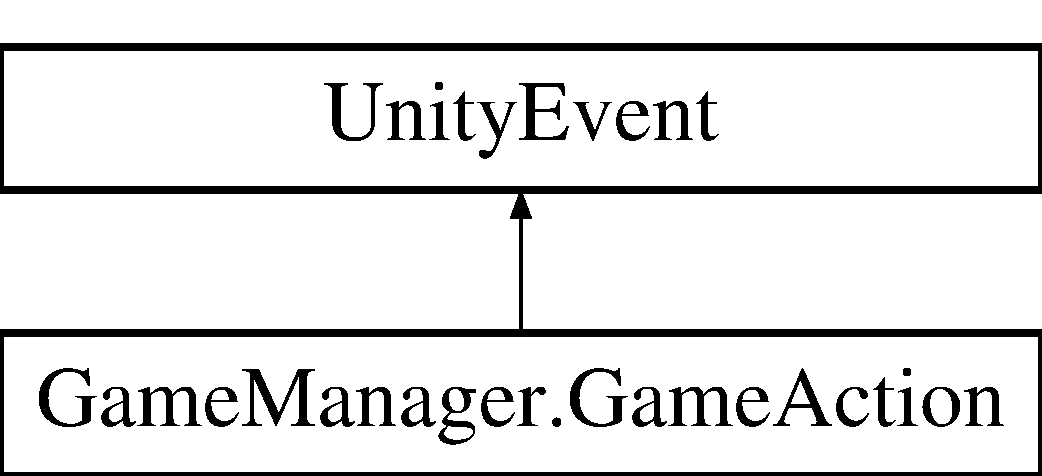
\includegraphics[height=2.000000cm]{class_game_manager_1_1_game_action}
\end{center}
\end{figure}


The documentation for this class was generated from the following file\-:\begin{DoxyCompactItemize}
\item 
/home/travis/build/temportalflux/\-Champ\-Net/\-Unity/\-Assets/\-Scripts/Game\-Manager.\-cs\end{DoxyCompactItemize}

\hypertarget{class_game_manager_1_1_game_action_flag}{\section{Game\-Manager.\-Game\-Action\-Flag Class Reference}
\label{class_game_manager_1_1_game_action_flag}\index{Game\-Manager.\-Game\-Action\-Flag@{Game\-Manager.\-Game\-Action\-Flag}}
}
Inheritance diagram for Game\-Manager.\-Game\-Action\-Flag\-:\begin{figure}[H]
\begin{center}
\leavevmode
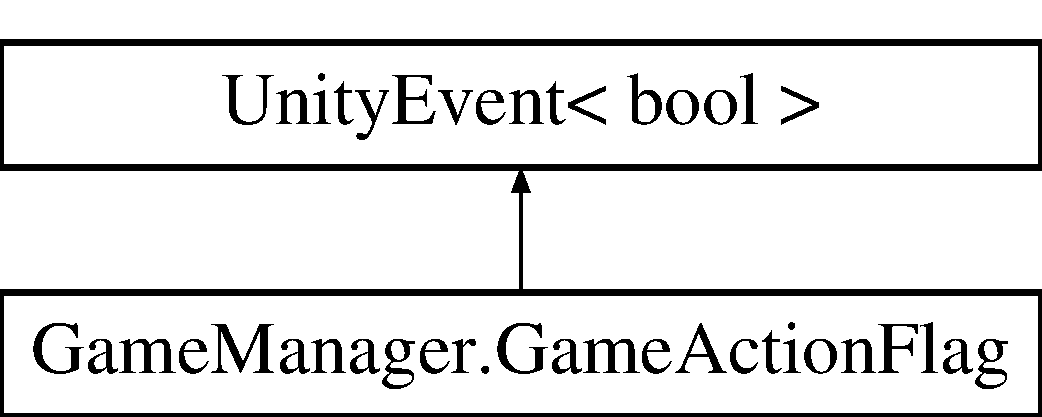
\includegraphics[height=2.000000cm]{class_game_manager_1_1_game_action_flag}
\end{center}
\end{figure}


The documentation for this class was generated from the following file\-:\begin{DoxyCompactItemize}
\item 
/home/travis/build/temportalflux/\-Champ\-Net/\-Unity/\-Assets/\-Scripts/Game\-Manager.\-cs\end{DoxyCompactItemize}

\hypertarget{class_game_manager_1_1_game_action_message}{\section{Game\-Manager.\-Game\-Action\-Message Class Reference}
\label{class_game_manager_1_1_game_action_message}\index{Game\-Manager.\-Game\-Action\-Message@{Game\-Manager.\-Game\-Action\-Message}}
}
Inheritance diagram for Game\-Manager.\-Game\-Action\-Message\-:\begin{figure}[H]
\begin{center}
\leavevmode
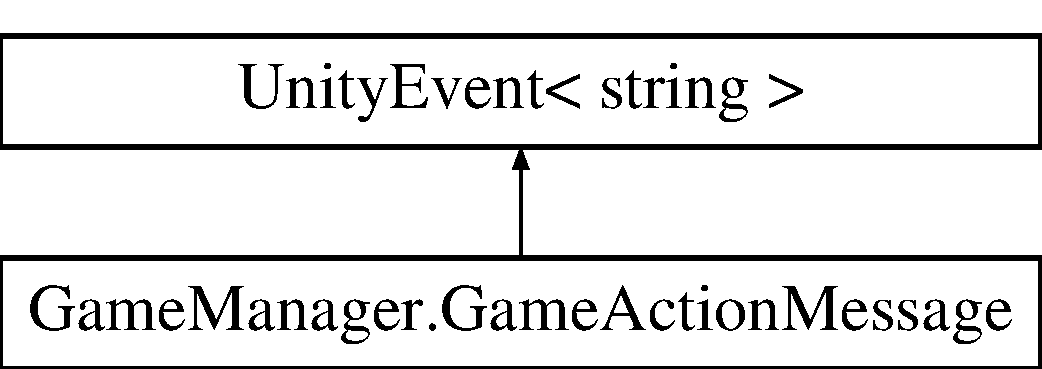
\includegraphics[height=2.000000cm]{class_game_manager_1_1_game_action_message}
\end{center}
\end{figure}


The documentation for this class was generated from the following file\-:\begin{DoxyCompactItemize}
\item 
/home/travis/build/temportalflux/\-Champ\-Net/\-Unity/\-Assets/\-Scripts/Game\-Manager.\-cs\end{DoxyCompactItemize}

\hypertarget{class_game_manager}{\section{Game\-Manager Class Reference}
\label{class_game_manager}\index{Game\-Manager@{Game\-Manager}}
}


The manager for the client game Is a singleton, instatiated in the first scene  


Inheritance diagram for Game\-Manager\-:\begin{figure}[H]
\begin{center}
\leavevmode
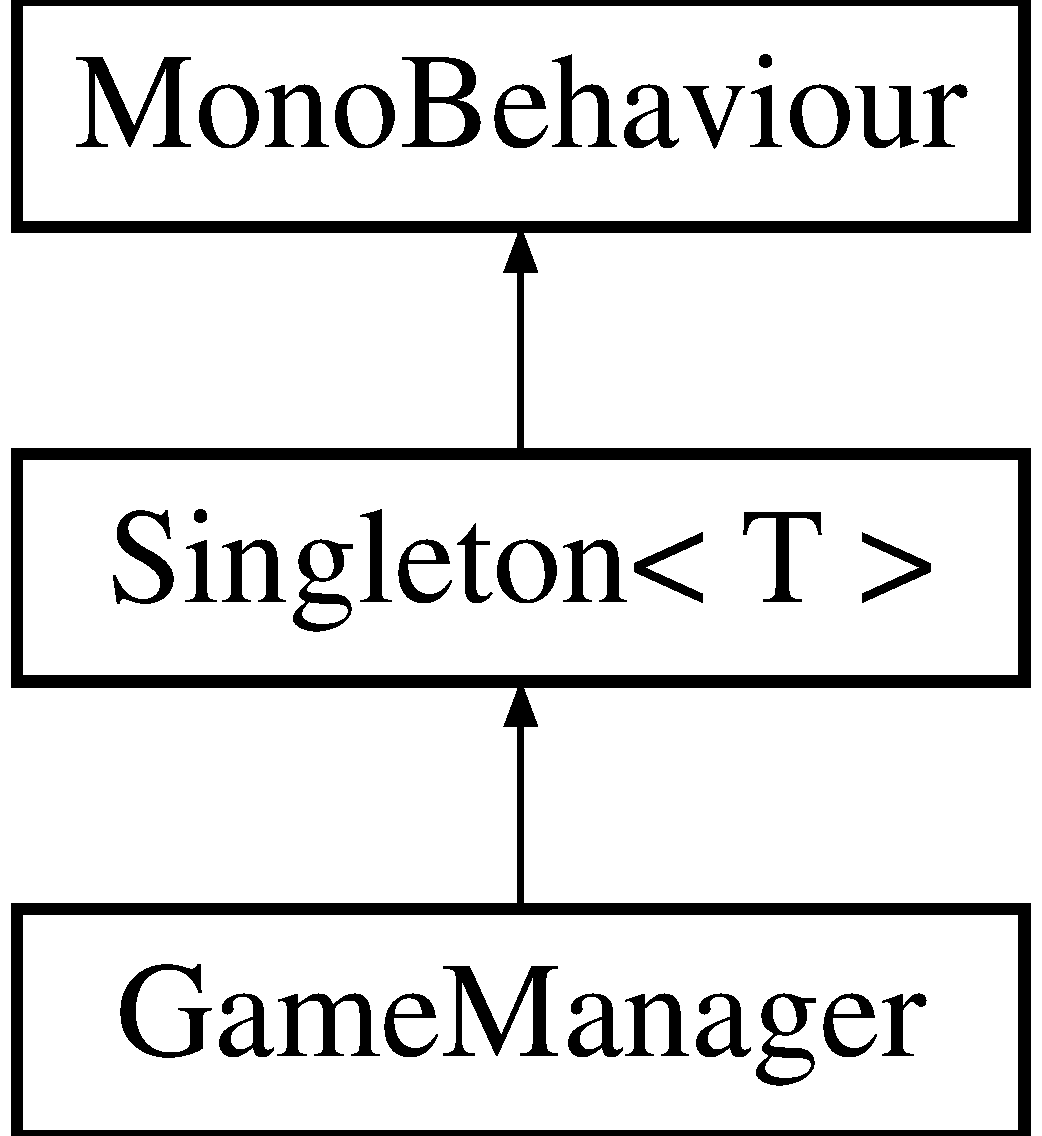
\includegraphics[height=3.000000cm]{class_game_manager}
\end{center}
\end{figure}
\subsection*{Classes}
\begin{DoxyCompactItemize}
\item 
class \hyperlink{class_game_manager_1_1_game_action}{Game\-Action}
\item 
class \hyperlink{class_game_manager_1_1_game_action_flag}{Game\-Action\-Flag}
\item 
class \hyperlink{class_game_manager_1_1_game_action_message}{Game\-Action\-Message}
\end{DoxyCompactItemize}
\subsection*{Public Member Functions}
\begin{DoxyCompactItemize}
\item 
void \hyperlink{class_game_manager_a3403831c40f16191e3997be60d95380b}{Play} ()
\begin{DoxyCompactList}\small\item\em Start the game in a local world \end{DoxyCompactList}\item 
void \hyperlink{class_game_manager_a1138f86278583414cba9456d02d0fa1c}{Play\-Network} ()
\begin{DoxyCompactList}\small\item\em Start the game in a networked world \end{DoxyCompactList}\item 
void \hyperlink{class_game_manager_a3c3a8e05664851d7642c13989af691cf}{Network\-Connect} (string address, int port, Connect\-Menu.\-Player\-Descriptor\mbox{[}$\,$\mbox{]} players)
\begin{DoxyCompactList}\small\item\em Connect the client with some server \end{DoxyCompactList}\item 
void \hyperlink{class_game_manager_a5d9cafdd495a4ed2760de13b7b9c80b6}{Exit} ()
\begin{DoxyCompactList}\small\item\em Exit the current scene \end{DoxyCompactList}\item 
\hyperlink{class_player_reference}{Player\-Reference} \hyperlink{class_game_manager_aadd5e389068b81b09036cc2bb8c097d6}{get\-Random\-Player} (\hyperlink{class_game_state_1_1_player}{Game\-State.\-Player} not\-Me)
\begin{DoxyCompactList}\small\item\em Get a random player from the current player listings in Game\-State.\-players \end{DoxyCompactList}\item 
Audio\-Source \hyperlink{class_game_manager_abf59d5ce551af5e35529f71a99d89d76}{Get\-Music\-Source} ()
\begin{DoxyCompactList}\small\item\em Gets the music source. \end{DoxyCompactList}\item 
\hypertarget{class_game_manager_a414dcfd0d1f5a5904d2440165e42923d}{void {\bfseries grab\-Score\-Board} ()}\label{class_game_manager_a414dcfd0d1f5a5904d2440165e42923d}

\item 
\hypertarget{class_game_manager_a9d3b6a3fb49a9402e1afde9224a12e21}{void {\bfseries Load\-Battle\-Scene} (\hyperlink{class_battle_participant}{Battle\-Participant} p1, \hyperlink{class_battle_participant}{Battle\-Participant} p2, bool is\-Netwoked\-Battle)}\label{class_game_manager_a9d3b6a3fb49a9402e1afde9224a12e21}

\item 
\hypertarget{class_game_manager_a4b49768a7f34b0f3795741f997eca643}{void {\bfseries Unload\-Battle\-Scene} ()}\label{class_game_manager_a4b49768a7f34b0f3795741f997eca643}

\end{DoxyCompactItemize}
\subsection*{Public Attributes}
\begin{DoxyCompactItemize}
\item 
\hypertarget{class_game_manager_a87d481fe88a1765f436ea5764cd1a21a}{\hyperlink{class_game_manager_1_1_game_action_flag}{Game\-Action\-Flag} {\bfseries on\-Network\-Connection\-Handled}}\label{class_game_manager_a87d481fe88a1765f436ea5764cd1a21a}

\item 
\hypertarget{class_game_manager_af977df043b83671ab9a4753b90fbf75b}{\hyperlink{class_game_manager_1_1_game_action_message}{Game\-Action\-Message} {\bfseries on\-Network\-Rejected}}\label{class_game_manager_af977df043b83671ab9a4753b90fbf75b}

\item 
\hyperlink{class_scene_transition}{Scene\-Transition} \hyperlink{class_game_manager_abae15982d4eb90ef9e5f3d24d15e22f2}{transition}
\begin{DoxyCompactList}\small\item\em The object to handle transitioning between scenes \end{DoxyCompactList}\item 
\hypertarget{class_game_manager_a57d400c7a28f42865048fbdbaf236cfb}{Game\-Object {\bfseries player\-Prefab}}\label{class_game_manager_a57d400c7a28f42865048fbdbaf236cfb}

\item 
\hyperlink{class_game_state}{Game\-State} \hyperlink{class_game_manager_a8d86b330237462e38933b28276ed0e2c}{state}
\begin{DoxyCompactList}\small\item\em The game state \end{DoxyCompactList}\item 
Main\-Camera \hyperlink{class_game_manager_aafd6b83529911d9e32cc4b79bd477d74}{main\-Camera}
\begin{DoxyCompactList}\small\item\em The main camera in the open-\/world \end{DoxyCompactList}\end{DoxyCompactItemize}
\subsection*{Properties}
\begin{DoxyCompactItemize}
\item 
static \hyperlink{class_game_manager}{Game\-Manager} \hyperlink{class_game_manager_a5c1d1f77dd4a2668a47a75c934c87075}{I\-N\-S\-T\-A\-N\-C\-E}\hspace{0.3cm}{\ttfamily  \mbox{[}get\mbox{]}}
\begin{DoxyCompactList}\small\item\em The public getter for the instance \end{DoxyCompactList}\end{DoxyCompactItemize}
\subsection*{Additional Inherited Members}


\subsection{Detailed Description}
The manager for the client game Is a singleton, instatiated in the first scene 

$<$author$>$Dustin Yost$<$/author$>$ 

\subsection{Member Function Documentation}
\hypertarget{class_game_manager_a5d9cafdd495a4ed2760de13b7b9c80b6}{\index{Game\-Manager@{Game\-Manager}!Exit@{Exit}}
\index{Exit@{Exit}!GameManager@{Game\-Manager}}
\subsubsection[{Exit}]{\setlength{\rightskip}{0pt plus 5cm}void Game\-Manager.\-Exit (
\begin{DoxyParamCaption}
{}
\end{DoxyParamCaption}
)\hspace{0.3cm}{\ttfamily [inline]}}}\label{class_game_manager_a5d9cafdd495a4ed2760de13b7b9c80b6}


Exit the current scene 

\hypertarget{class_game_manager_abf59d5ce551af5e35529f71a99d89d76}{\index{Game\-Manager@{Game\-Manager}!Get\-Music\-Source@{Get\-Music\-Source}}
\index{Get\-Music\-Source@{Get\-Music\-Source}!GameManager@{Game\-Manager}}
\subsubsection[{Get\-Music\-Source}]{\setlength{\rightskip}{0pt plus 5cm}Audio\-Source Game\-Manager.\-Get\-Music\-Source (
\begin{DoxyParamCaption}
{}
\end{DoxyParamCaption}
)\hspace{0.3cm}{\ttfamily [inline]}}}\label{class_game_manager_abf59d5ce551af5e35529f71a99d89d76}


Gets the music source. 

\begin{DoxyReturn}{Returns}
The Audio\-Source component
\end{DoxyReturn}
\hypertarget{class_game_manager_aadd5e389068b81b09036cc2bb8c097d6}{\index{Game\-Manager@{Game\-Manager}!get\-Random\-Player@{get\-Random\-Player}}
\index{get\-Random\-Player@{get\-Random\-Player}!GameManager@{Game\-Manager}}
\subsubsection[{get\-Random\-Player}]{\setlength{\rightskip}{0pt plus 5cm}{\bf Player\-Reference} Game\-Manager.\-get\-Random\-Player (
\begin{DoxyParamCaption}
\item[{{\bf Game\-State.\-Player}}]{not\-Me}
\end{DoxyParamCaption}
)\hspace{0.3cm}{\ttfamily [inline]}}}\label{class_game_manager_aadd5e389068b81b09036cc2bb8c097d6}


Get a random player from the current player listings in Game\-State.\-players 


\begin{DoxyParams}{Parameters}
{\em not\-Me} & The player which should not be included\\
\hline
\end{DoxyParams}
\begin{DoxyReturn}{Returns}

\end{DoxyReturn}
\hypertarget{class_game_manager_a3c3a8e05664851d7642c13989af691cf}{\index{Game\-Manager@{Game\-Manager}!Network\-Connect@{Network\-Connect}}
\index{Network\-Connect@{Network\-Connect}!GameManager@{Game\-Manager}}
\subsubsection[{Network\-Connect}]{\setlength{\rightskip}{0pt plus 5cm}void Game\-Manager.\-Network\-Connect (
\begin{DoxyParamCaption}
\item[{string}]{address, }
\item[{int}]{port, }
\item[{Connect\-Menu.\-Player\-Descriptor\mbox{[}$\,$\mbox{]}}]{players}
\end{DoxyParamCaption}
)\hspace{0.3cm}{\ttfamily [inline]}}}\label{class_game_manager_a3c3a8e05664851d7642c13989af691cf}


Connect the client with some server 


\begin{DoxyParams}{Parameters}
{\em address} & The I\-Pv4 address\\
\hline
{\em port} & The address port\\
\hline
{\em players} & the desired player descriptors to connect with\\
\hline
\end{DoxyParams}
\hypertarget{class_game_manager_a3403831c40f16191e3997be60d95380b}{\index{Game\-Manager@{Game\-Manager}!Play@{Play}}
\index{Play@{Play}!GameManager@{Game\-Manager}}
\subsubsection[{Play}]{\setlength{\rightskip}{0pt plus 5cm}void Game\-Manager.\-Play (
\begin{DoxyParamCaption}
{}
\end{DoxyParamCaption}
)\hspace{0.3cm}{\ttfamily [inline]}}}\label{class_game_manager_a3403831c40f16191e3997be60d95380b}


Start the game in a local world 

\hypertarget{class_game_manager_a1138f86278583414cba9456d02d0fa1c}{\index{Game\-Manager@{Game\-Manager}!Play\-Network@{Play\-Network}}
\index{Play\-Network@{Play\-Network}!GameManager@{Game\-Manager}}
\subsubsection[{Play\-Network}]{\setlength{\rightskip}{0pt plus 5cm}void Game\-Manager.\-Play\-Network (
\begin{DoxyParamCaption}
{}
\end{DoxyParamCaption}
)\hspace{0.3cm}{\ttfamily [inline]}}}\label{class_game_manager_a1138f86278583414cba9456d02d0fa1c}


Start the game in a networked world 



\subsection{Member Data Documentation}
\hypertarget{class_game_manager_aafd6b83529911d9e32cc4b79bd477d74}{\index{Game\-Manager@{Game\-Manager}!main\-Camera@{main\-Camera}}
\index{main\-Camera@{main\-Camera}!GameManager@{Game\-Manager}}
\subsubsection[{main\-Camera}]{\setlength{\rightskip}{0pt plus 5cm}Main\-Camera Game\-Manager.\-main\-Camera}}\label{class_game_manager_aafd6b83529911d9e32cc4b79bd477d74}


The main camera in the open-\/world 

\hypertarget{class_game_manager_a8d86b330237462e38933b28276ed0e2c}{\index{Game\-Manager@{Game\-Manager}!state@{state}}
\index{state@{state}!GameManager@{Game\-Manager}}
\subsubsection[{state}]{\setlength{\rightskip}{0pt plus 5cm}{\bf Game\-State} Game\-Manager.\-state}}\label{class_game_manager_a8d86b330237462e38933b28276ed0e2c}


The game state 

\hypertarget{class_game_manager_abae15982d4eb90ef9e5f3d24d15e22f2}{\index{Game\-Manager@{Game\-Manager}!transition@{transition}}
\index{transition@{transition}!GameManager@{Game\-Manager}}
\subsubsection[{transition}]{\setlength{\rightskip}{0pt plus 5cm}{\bf Scene\-Transition} Game\-Manager.\-transition}}\label{class_game_manager_abae15982d4eb90ef9e5f3d24d15e22f2}


The object to handle transitioning between scenes 



\subsection{Property Documentation}
\hypertarget{class_game_manager_a5c1d1f77dd4a2668a47a75c934c87075}{\index{Game\-Manager@{Game\-Manager}!I\-N\-S\-T\-A\-N\-C\-E@{I\-N\-S\-T\-A\-N\-C\-E}}
\index{I\-N\-S\-T\-A\-N\-C\-E@{I\-N\-S\-T\-A\-N\-C\-E}!GameManager@{Game\-Manager}}
\subsubsection[{I\-N\-S\-T\-A\-N\-C\-E}]{\setlength{\rightskip}{0pt plus 5cm}{\bf Game\-Manager} Game\-Manager.\-I\-N\-S\-T\-A\-N\-C\-E\hspace{0.3cm}{\ttfamily [static]}, {\ttfamily [get]}}}\label{class_game_manager_a5c1d1f77dd4a2668a47a75c934c87075}


The public getter for the instance 



The documentation for this class was generated from the following file\-:\begin{DoxyCompactItemize}
\item 
/home/travis/build/temportalflux/\-Champ\-Net/\-Unity/\-Assets/\-Scripts/Game\-Manager.\-cs\end{DoxyCompactItemize}

\hypertarget{class_game_state}{\section{Game\-State Class Reference}
\label{class_game_state}\index{Game\-State@{Game\-State}}
}


Holds all persistent data from network intergration for local usage  


Inheritance diagram for Game\-State\-:\begin{figure}[H]
\begin{center}
\leavevmode
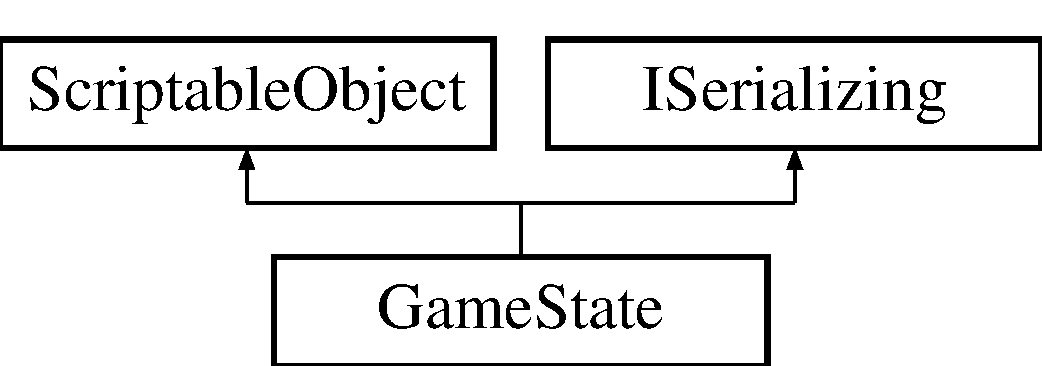
\includegraphics[height=2.000000cm]{class_game_state}
\end{center}
\end{figure}
\subsection*{Classes}
\begin{DoxyCompactItemize}
\item 
struct \hyperlink{class_game_state_1_1_player}{Player}
\begin{DoxyCompactList}\small\item\em A state class for all \hyperlink{class_game_state_1_1_player}{Player} objects \end{DoxyCompactList}\end{DoxyCompactItemize}
\subsection*{Public Member Functions}
\begin{DoxyCompactItemize}
\item 
\hypertarget{class_game_state_a05acc40696378ba026165a2cc824acf0}{bool {\bfseries Has\-Player} (ref \hyperlink{class_game_state_1_1_player}{Player} info)}\label{class_game_state_a05acc40696378ba026165a2cc824acf0}

\item 
void \hyperlink{class_game_state_a4c4e32237639764263332c7c236974d1}{Add\-Player} (\hyperlink{class_game_state_1_1_player}{Player} info)
\begin{DoxyCompactList}\small\item\em Add a player to the current game object scene via its info \end{DoxyCompactList}\item 
\hypertarget{class_game_state_ae8d21ce826daada0dabeadd11c6eb233}{void {\bfseries Remove\-Player} (\hyperlink{class_game_state_1_1_player}{Player} info)}\label{class_game_state_ae8d21ce826daada0dabeadd11c6eb233}

\item 
\hypertarget{class_game_state_a1e3c3340e55693af1c8326879a81f1c4}{void {\bfseries Add\-Player\-Local} (\hyperlink{class_game_state_1_1_player}{Player} info)}\label{class_game_state_a1e3c3340e55693af1c8326879a81f1c4}

\item 
\hypertarget{class_game_state_a2e6cdef311e93ec46d07206d621f6837}{void {\bfseries Add\-Player\-Connected} (\hyperlink{class_game_state_1_1_player}{Player} info)}\label{class_game_state_a2e6cdef311e93ec46d07206d621f6837}

\item 
\hypertarget{class_game_state_a61e4817740bd283ce4a6ea44e0d0f00a}{void {\bfseries Spawn\-Local\-Multiplayer} ()}\label{class_game_state_a61e4817740bd283ce4a6ea44e0d0f00a}

\item 
\hypertarget{class_game_state_a82b88c45043a403441d3eef1e0b72266}{void {\bfseries Spawn\-Local\-Player} ()}\label{class_game_state_a82b88c45043a403441d3eef1e0b72266}

\item 
\hypertarget{class_game_state_af2fbb55979f8cc6da50317e1d701e370}{void {\bfseries Spawn\-Player} ()}\label{class_game_state_af2fbb55979f8cc6da50317e1d701e370}

\item 
int \hyperlink{class_game_state_a57d152b243c11aa86e7ba0f07b4bd0dd}{Get\-Size} ()
\begin{DoxyCompactList}\small\item\em Returns the size of the packet (the size for a potential byte\mbox{[}\mbox{]}) \end{DoxyCompactList}\item 
void \hyperlink{class_game_state_af57a06c77a763e8b57841bab79c9b12f}{Serialize} (ref byte\mbox{[}$\,$\mbox{]} data, ref int last\-Index)
\begin{DoxyCompactList}\small\item\em Serializes data from this event into a byte array. Unused for \hyperlink{class_game_state}{Game\-State}. Game\-States are O\-N\-L\-Y serialized via server. \end{DoxyCompactList}\item 
void \hyperlink{class_game_state_aa5f956de2c49182fbe5fc32e9d2ca431}{Deserialize} (byte\mbox{[}$\,$\mbox{]} data, ref int last\-Index)
\begin{DoxyCompactList}\small\item\em Deserializes data from a byte array into this event's data \end{DoxyCompactList}\item 
\hypertarget{class_game_state_a268b639f06e4fa7fa1ca1819cc5d3175}{void {\bfseries Fixed\-Update} ()}\label{class_game_state_a268b639f06e4fa7fa1ca1819cc5d3175}

\item 
\hypertarget{class_game_state_a74a35fb7045c0eee7e68f07c387e2ddf}{{\bfseries Game\-State} (int id)}\label{class_game_state_a74a35fb7045c0eee7e68f07c387e2ddf}

\item 
\hypertarget{class_game_state_ad74bf5767b052d5b32805220ca0c1fab}{void {\bfseries add\-Player} (unsigned int \hyperlink{class_game_state_ad24a423ba6655fc6541b2f12ce98e0d0}{client\-I\-D}, unsigned int player\-I\-D, unsigned int local\-I\-D, std\-::string name, float color\-R, float color\-G, float color\-B)}\label{class_game_state_ad74bf5767b052d5b32805220ca0c1fab}

\item 
\hypertarget{class_game_state_a733fa68895adba783b0b4b804f16906f}{void {\bfseries remove\-Player} (unsigned int player\-I\-D)}\label{class_game_state_a733fa68895adba783b0b4b804f16906f}

\item 
\hypertarget{class_game_state_a291fcda337b1a25c21871fe338399c27}{char $\ast$ {\bfseries serialize\-For\-Client} (unsigned char packet\-I\-D, int \hyperlink{class_game_state_ad24a423ba6655fc6541b2f12ce98e0d0}{client\-I\-D}, int \&data\-Length)}\label{class_game_state_a291fcda337b1a25c21871fe338399c27}

\end{DoxyCompactItemize}
\subsection*{Static Public Member Functions}
\begin{DoxyCompactItemize}
\item 
static void \hyperlink{class_game_state_a2f3154927e33e16bd595b4aece996c61}{Create} ()
\begin{DoxyCompactList}\small\item\em Creates a Scriptable\-Object for \hyperlink{class_game_state}{Game\-State} from a Unity Menu context \end{DoxyCompactList}\end{DoxyCompactItemize}
\subsection*{Public Attributes}
\begin{DoxyCompactItemize}
\item 
Connect\-Menu.\-Player\-Descriptor\mbox{[}$\,$\mbox{]} \hyperlink{class_game_state_a8b1949523ac8e40776c0617666023d64}{player\-Request} = null
\begin{DoxyCompactList}\small\item\em Not Serialized. Used to store the requests for players on world-\/enter \end{DoxyCompactList}\item 
\hypertarget{class_game_state_ad68ed3f1f32060bfff68d296e6750712}{bool {\bfseries editor\-Foldout\-Players}}\label{class_game_state_ad68ed3f1f32060bfff68d296e6750712}

\item 
\hypertarget{class_game_state_a47358e83d829da7a28c49f8d0a795125}{Dictionary$<$ I\-D, bool $>$ {\bfseries editor\-Foldouts}}\label{class_game_state_a47358e83d829da7a28c49f8d0a795125}

\item 
\hypertarget{class_game_state_aa4cba70bc38a13e80439dc784c6ca12e}{bool {\bfseries is\-Local\-Game}}\label{class_game_state_aa4cba70bc38a13e80439dc784c6ca12e}

\item 
uint \hyperlink{class_game_state_ad24a423ba6655fc6541b2f12ce98e0d0}{client\-I\-D}
\begin{DoxyCompactList}\small\item\em A unique identifier (across all peers in the network) of the client which controls this player \end{DoxyCompactList}\item 
\hypertarget{class_game_state_a3d88394849f2356b1c1917f8bb9cc873}{\hyperlink{class_monster_data_object}{Monster\-Data\-Object}\mbox{[}$\,$\mbox{]} {\bfseries starters}}\label{class_game_state_a3d88394849f2356b1c1917f8bb9cc873}

\item 
\hypertarget{class_game_state_a857eed8c97274c3dd9d3eb558a33f855}{float {\bfseries delta\-Time}}\label{class_game_state_a857eed8c97274c3dd9d3eb558a33f855}

\item 
\hypertarget{class_game_state_aed9c4cf83c497c6e36585e0ed3999564}{Dictionary$<$ I\-D, \hyperlink{class_game_state_1_1_player}{Player} $>$ {\bfseries players}}\label{class_game_state_aed9c4cf83c497c6e36585e0ed3999564}

\item 
\hypertarget{class_game_state_adb8c9c7f10d683332cbd62927d35cb35}{int {\bfseries client\-I\-D}}\label{class_game_state_adb8c9c7f10d683332cbd62927d35cb35}

\item 
\hypertarget{class_game_state_a8f156a6cce5f2b9945c274b6bfc971ce}{std\-::map$<$ unsigned int, \hyperlink{class_game_state_1_1_player}{Player} $>$ {\bfseries players}}\label{class_game_state_a8f156a6cce5f2b9945c274b6bfc971ce}

\end{DoxyCompactItemize}
\subsection*{Properties}
\begin{DoxyCompactItemize}
\item 
\hypertarget{class_game_state_a3fe38a9e11fe72dd4bc4796e1d4a6c1b}{Dictionary$<$ uint, \hyperlink{class_game_state_1_1_player}{Player} $>$ {\bfseries local\-Players}\hspace{0.3cm}{\ttfamily  \mbox{[}get\mbox{]}}}\label{class_game_state_a3fe38a9e11fe72dd4bc4796e1d4a6c1b}

\item 
\hypertarget{class_game_state_ad0f225ac26f38bf21be10d35a1cd6011}{Dictionary$<$ uint, \hyperlink{class_game_state_1_1_player}{Player} $>$ {\bfseries connected\-Players}\hspace{0.3cm}{\ttfamily  \mbox{[}get\mbox{]}}}\label{class_game_state_ad0f225ac26f38bf21be10d35a1cd6011}

\end{DoxyCompactItemize}


\subsection{Detailed Description}
Holds all persistent data from network intergration for local usage 

\begin{DoxyAuthor}{Author}
Dustin Yost 
\end{DoxyAuthor}


\subsection{Member Function Documentation}
\hypertarget{class_game_state_a4c4e32237639764263332c7c236974d1}{\index{Game\-State@{Game\-State}!Add\-Player@{Add\-Player}}
\index{Add\-Player@{Add\-Player}!GameState@{Game\-State}}
\subsubsection[{Add\-Player}]{\setlength{\rightskip}{0pt plus 5cm}void Game\-State.\-Add\-Player (
\begin{DoxyParamCaption}
\item[{{\bf Player}}]{info}
\end{DoxyParamCaption}
)\hspace{0.3cm}{\ttfamily [inline]}}}\label{class_game_state_a4c4e32237639764263332c7c236974d1}


Add a player to the current game object scene via its info 


\begin{DoxyParams}{Parameters}
{\em info} & \\
\hline
\end{DoxyParams}
\hypertarget{class_game_state_a2f3154927e33e16bd595b4aece996c61}{\index{Game\-State@{Game\-State}!Create@{Create}}
\index{Create@{Create}!GameState@{Game\-State}}
\subsubsection[{Create}]{\setlength{\rightskip}{0pt plus 5cm}static void Game\-State.\-Create (
\begin{DoxyParamCaption}
{}
\end{DoxyParamCaption}
)\hspace{0.3cm}{\ttfamily [inline]}, {\ttfamily [static]}}}\label{class_game_state_a2f3154927e33e16bd595b4aece996c61}


Creates a Scriptable\-Object for \hyperlink{class_game_state}{Game\-State} from a Unity Menu context 

\hypertarget{class_game_state_aa5f956de2c49182fbe5fc32e9d2ca431}{\index{Game\-State@{Game\-State}!Deserialize@{Deserialize}}
\index{Deserialize@{Deserialize}!GameState@{Game\-State}}
\subsubsection[{Deserialize}]{\setlength{\rightskip}{0pt plus 5cm}void Game\-State.\-Deserialize (
\begin{DoxyParamCaption}
\item[{byte\mbox{[}$\,$\mbox{]}}]{data, }
\item[{ref int}]{last\-Index}
\end{DoxyParamCaption}
)\hspace{0.3cm}{\ttfamily [inline]}}}\label{class_game_state_aa5f956de2c49182fbe5fc32e9d2ca431}


Deserializes data from a byte array into this event's data 


\begin{DoxyParams}{Parameters}
{\em data} & The data.\\
\hline
{\em last\-Index} & The last index.\\
\hline
\end{DoxyParams}
\begin{DoxyAuthor}{Author}
Dustin Yost 
\end{DoxyAuthor}


Implements \hyperlink{interface_i_serializing_a92f8ba3a06d21e7b01e37411e4e3145c}{I\-Serializing}.

\hypertarget{class_game_state_a57d152b243c11aa86e7ba0f07b4bd0dd}{\index{Game\-State@{Game\-State}!Get\-Size@{Get\-Size}}
\index{Get\-Size@{Get\-Size}!GameState@{Game\-State}}
\subsubsection[{Get\-Size}]{\setlength{\rightskip}{0pt plus 5cm}int Game\-State.\-Get\-Size (
\begin{DoxyParamCaption}
{}
\end{DoxyParamCaption}
)\hspace{0.3cm}{\ttfamily [inline]}}}\label{class_game_state_a57d152b243c11aa86e7ba0f07b4bd0dd}


Returns the size of the packet (the size for a potential byte\mbox{[}\mbox{]}) 

\begin{DoxyReturn}{Returns}
the integer length of a byte array to hold this event's data 
\end{DoxyReturn}


Author\-: Dustin Yost 

Implements \hyperlink{interface_i_serializing_a9e6ea0afaeac8d1d57e20579f87bebe2}{I\-Serializing}.

\hypertarget{class_game_state_af57a06c77a763e8b57841bab79c9b12f}{\index{Game\-State@{Game\-State}!Serialize@{Serialize}}
\index{Serialize@{Serialize}!GameState@{Game\-State}}
\subsubsection[{Serialize}]{\setlength{\rightskip}{0pt plus 5cm}void Game\-State.\-Serialize (
\begin{DoxyParamCaption}
\item[{ref byte\mbox{[}$\,$\mbox{]}}]{data, }
\item[{ref int}]{last\-Index}
\end{DoxyParamCaption}
)\hspace{0.3cm}{\ttfamily [inline]}}}\label{class_game_state_af57a06c77a763e8b57841bab79c9b12f}


Serializes data from this event into a byte array. Unused for \hyperlink{class_game_state}{Game\-State}. Game\-States are O\-N\-L\-Y serialized via server. 


\begin{DoxyParams}{Parameters}
{\em data} & The data.\\
\hline
{\em last\-Index} & The last index.\\
\hline
\end{DoxyParams}
\begin{DoxyAuthor}{Author}
Dustin Yost 
\end{DoxyAuthor}


Implements \hyperlink{interface_i_serializing_ac31a44c2358a197e774fa3f79cc80356}{I\-Serializing}.



\subsection{Member Data Documentation}
\hypertarget{class_game_state_ad24a423ba6655fc6541b2f12ce98e0d0}{\index{Game\-State@{Game\-State}!client\-I\-D@{client\-I\-D}}
\index{client\-I\-D@{client\-I\-D}!GameState@{Game\-State}}
\subsubsection[{client\-I\-D}]{\setlength{\rightskip}{0pt plus 5cm}uint Game\-State.\-client\-I\-D}}\label{class_game_state_ad24a423ba6655fc6541b2f12ce98e0d0}


A unique identifier (across all peers in the network) of the client which controls this player 

\hypertarget{class_game_state_a8b1949523ac8e40776c0617666023d64}{\index{Game\-State@{Game\-State}!player\-Request@{player\-Request}}
\index{player\-Request@{player\-Request}!GameState@{Game\-State}}
\subsubsection[{player\-Request}]{\setlength{\rightskip}{0pt plus 5cm}Connect\-Menu.\-Player\-Descriptor \mbox{[}$\,$\mbox{]} Game\-State.\-player\-Request = null}}\label{class_game_state_a8b1949523ac8e40776c0617666023d64}


Not Serialized. Used to store the requests for players on world-\/enter 



The documentation for this class was generated from the following files\-:\begin{DoxyCompactItemize}
\item 
/home/travis/build/temportalflux/\-Champ\-Net/\-Unity/\-Assets/\-Scripts/Game\-State.\-cs\item 
/home/travis/build/temportalflux/\-Champ\-Net/\-Champ\-Net/\-Champ\-Net\-Plugin\-Test/include/Game\-State.\-h\item 
/home/travis/build/temportalflux/\-Champ\-Net/\-Champ\-Net/\-Champ\-Net\-Plugin\-Test/source/Game\-State.\-cpp\end{DoxyCompactItemize}

\hypertarget{class_monster_data_object}{\section{Monster\-Data\-Object Class Reference}
\label{class_monster_data_object}\index{Monster\-Data\-Object@{Monster\-Data\-Object}}
}
\subsection*{Public Member Functions}
\begin{DoxyCompactItemize}
\item 
int \hyperlink{class_monster_data_object_a6dd85baaa39abaac720a36b71db7536e}{Get\-Monster\-Attack\-Stat} (Move\-Kind physical\-Or\-Special, bool apply\-Stat\-Stages=false)
\begin{DoxyCompactList}\small\item\em Get the attack stat based on the move kind \end{DoxyCompactList}\item 
int \hyperlink{class_monster_data_object_a1eda550eeb621625d872b66b1c27eba7}{Get\-Monster\-Defense\-Stat} (Move\-Kind physical\-Or\-Special, bool apply\-Stat\-Stages=false)
\begin{DoxyCompactList}\small\item\em Get the defense stat based on the move kind. \end{DoxyCompactList}\end{DoxyCompactItemize}
\subsection*{Public Attributes}
\begin{DoxyCompactItemize}
\item 
\hypertarget{class_monster_data_object_a32f219c168636419992aa379f59c9ff0}{\hyperlink{class_monster_stat}{Monster\-Stat} {\bfseries monster\-Stat}}\label{class_monster_data_object_a32f219c168636419992aa379f59c9ff0}

\item 
\hypertarget{class_monster_data_object_ac1197136faf77c440906bade6ee2b690}{int {\bfseries stat\-Stage\-Attack}}\label{class_monster_data_object_ac1197136faf77c440906bade6ee2b690}

\item 
\hypertarget{class_monster_data_object_a0a292ad39496e69386b877f3ddaeb123}{int {\bfseries stat\-Stage\-Defense}}\label{class_monster_data_object_a0a292ad39496e69386b877f3ddaeb123}

\item 
\hypertarget{class_monster_data_object_a70677e28a5a8ba6ae3a2cad0ffdb0c47}{int {\bfseries stat\-Stage\-Special\-Attack}}\label{class_monster_data_object_a70677e28a5a8ba6ae3a2cad0ffdb0c47}

\item 
\hypertarget{class_monster_data_object_a1aca4196d55b289763cced6b55b2ddc8}{int {\bfseries stat\-Stage\-Special\-Defense}}\label{class_monster_data_object_a1aca4196d55b289763cced6b55b2ddc8}

\item 
\hypertarget{class_monster_data_object_a6572a7633fc1cd965e2c6c0ab7b86f9f}{int {\bfseries stat\-Stage\-Speed}}\label{class_monster_data_object_a6572a7633fc1cd965e2c6c0ab7b86f9f}

\end{DoxyCompactItemize}
\subsection*{Properties}
\begin{DoxyCompactItemize}
\item 
\hypertarget{class_monster_data_object_a6c67d5bab62fb649e01355b52ccf16ba}{string {\bfseries Get\-Monster\-Name}\hspace{0.3cm}{\ttfamily  \mbox{[}get\mbox{]}}}\label{class_monster_data_object_a6c67d5bab62fb649e01355b52ccf16ba}

\item 
\hypertarget{class_monster_data_object_a0d1ed24b79b82bb78c26811aa34b3ac7}{List$<$ Monster\-Type $>$ {\bfseries Get\-Types}\hspace{0.3cm}{\ttfamily  \mbox{[}get\mbox{]}}}\label{class_monster_data_object_a0d1ed24b79b82bb78c26811aa34b3ac7}

\item 
\hypertarget{class_monster_data_object_ae1c3d104809049c612c9a1b6a61664be}{int {\bfseries Get\-Attack}\hspace{0.3cm}{\ttfamily  \mbox{[}get\mbox{]}}}\label{class_monster_data_object_ae1c3d104809049c612c9a1b6a61664be}

\item 
\hypertarget{class_monster_data_object_a2409f379ef651b10b5d7638154da7421}{int {\bfseries Get\-Defense}\hspace{0.3cm}{\ttfamily  \mbox{[}get\mbox{]}}}\label{class_monster_data_object_a2409f379ef651b10b5d7638154da7421}

\item 
\hypertarget{class_monster_data_object_a5beec2bbced5d78744aa0ea784218357}{int {\bfseries Get\-Special\-Attack}\hspace{0.3cm}{\ttfamily  \mbox{[}get\mbox{]}}}\label{class_monster_data_object_a5beec2bbced5d78744aa0ea784218357}

\item 
\hypertarget{class_monster_data_object_aafcc2ea03b96291140ebcb40331e4cd2}{int {\bfseries Get\-Special\-Defense}\hspace{0.3cm}{\ttfamily  \mbox{[}get\mbox{]}}}\label{class_monster_data_object_aafcc2ea03b96291140ebcb40331e4cd2}

\item 
\hypertarget{class_monster_data_object_a0d7639dc92ae01942b1b996565eff2ae}{int {\bfseries Get\-Speed}\hspace{0.3cm}{\ttfamily  \mbox{[}get\mbox{]}}}\label{class_monster_data_object_a0d7639dc92ae01942b1b996565eff2ae}

\item 
\hypertarget{class_monster_data_object_aced78f5f04d3dbb79a0f8291fbe118bd}{List$<$ \hyperlink{class_attack_object}{Attack\-Object} $>$ {\bfseries Get\-Available\-Attacks}\hspace{0.3cm}{\ttfamily  \mbox{[}get\mbox{]}}}\label{class_monster_data_object_aced78f5f04d3dbb79a0f8291fbe118bd}

\end{DoxyCompactItemize}


\subsection{Member Function Documentation}
\hypertarget{class_monster_data_object_a6dd85baaa39abaac720a36b71db7536e}{\index{Monster\-Data\-Object@{Monster\-Data\-Object}!Get\-Monster\-Attack\-Stat@{Get\-Monster\-Attack\-Stat}}
\index{Get\-Monster\-Attack\-Stat@{Get\-Monster\-Attack\-Stat}!MonsterDataObject@{Monster\-Data\-Object}}
\subsubsection[{Get\-Monster\-Attack\-Stat}]{\setlength{\rightskip}{0pt plus 5cm}int Monster\-Data\-Object.\-Get\-Monster\-Attack\-Stat (
\begin{DoxyParamCaption}
\item[{Move\-Kind}]{physical\-Or\-Special, }
\item[{bool}]{apply\-Stat\-Stages = {\ttfamily false}}
\end{DoxyParamCaption}
)\hspace{0.3cm}{\ttfamily [inline]}}}\label{class_monster_data_object_a6dd85baaa39abaac720a36b71db7536e}


Get the attack stat based on the move kind 


\begin{DoxyParams}{Parameters}
{\em physical\-Or\-Special} & is the move physical or special?\\
\hline
{\em apply\-Stat\-Stages} & if {\ttfamily true} then the stat stages are applied\\
\hline
\end{DoxyParams}
\begin{DoxyReturn}{Returns}
the modified attack stat
\end{DoxyReturn}
\hypertarget{class_monster_data_object_a1eda550eeb621625d872b66b1c27eba7}{\index{Monster\-Data\-Object@{Monster\-Data\-Object}!Get\-Monster\-Defense\-Stat@{Get\-Monster\-Defense\-Stat}}
\index{Get\-Monster\-Defense\-Stat@{Get\-Monster\-Defense\-Stat}!MonsterDataObject@{Monster\-Data\-Object}}
\subsubsection[{Get\-Monster\-Defense\-Stat}]{\setlength{\rightskip}{0pt plus 5cm}int Monster\-Data\-Object.\-Get\-Monster\-Defense\-Stat (
\begin{DoxyParamCaption}
\item[{Move\-Kind}]{physical\-Or\-Special, }
\item[{bool}]{apply\-Stat\-Stages = {\ttfamily false}}
\end{DoxyParamCaption}
)\hspace{0.3cm}{\ttfamily [inline]}}}\label{class_monster_data_object_a1eda550eeb621625d872b66b1c27eba7}


Get the defense stat based on the move kind. 


\begin{DoxyParams}{Parameters}
{\em physical\-Or\-Special} & is the move physical or special?\\
\hline
{\em apply\-Stat\-Stages} & if {\ttfamily true} then the stat stages are applied\\
\hline
\end{DoxyParams}
\begin{DoxyReturn}{Returns}
the modified defense stat
\end{DoxyReturn}


The documentation for this class was generated from the following file\-:\begin{DoxyCompactItemize}
\item 
/home/travis/build/temportalflux/\-Champ\-Net/\-Unity/\-Assets/\-Scripts/Monster\-Data\-Object.\-cs\end{DoxyCompactItemize}

\hypertarget{struct_game_state_1_1_player}{\section{Game\-State.\-Player Struct Reference}
\label{struct_game_state_1_1_player}\index{Game\-State.\-Player@{Game\-State.\-Player}}
}
Inheritance diagram for Game\-State.\-Player\-:\begin{figure}[H]
\begin{center}
\leavevmode
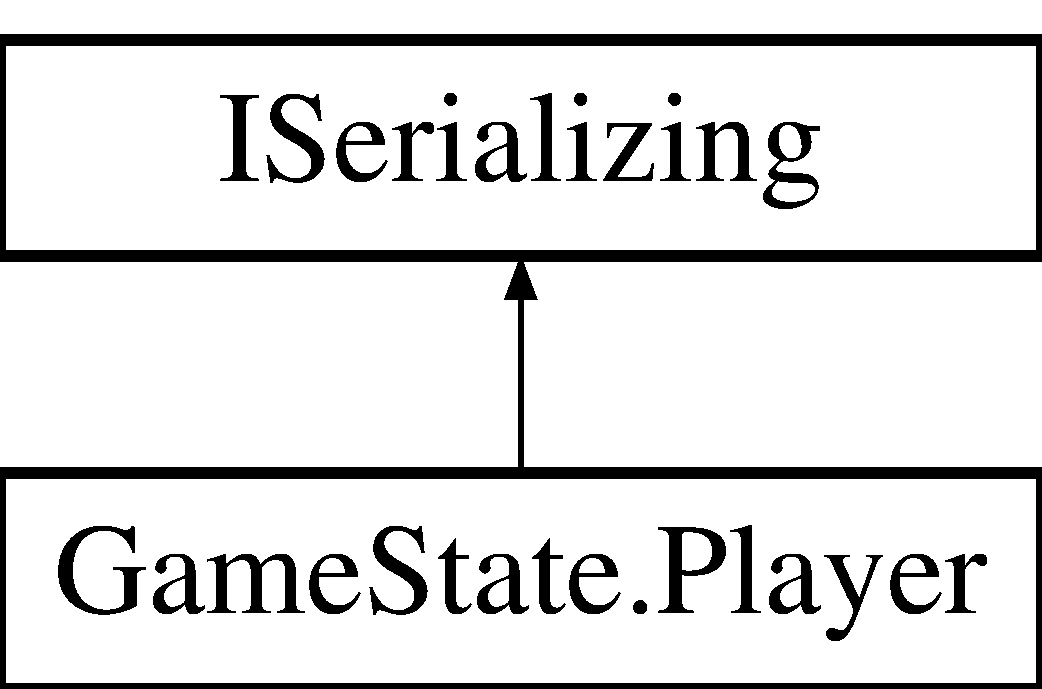
\includegraphics[height=2.000000cm]{struct_game_state_1_1_player}
\end{center}
\end{figure}
\subsection*{Public Types}
\begin{DoxyCompactItemize}
\item 
enum \hyperlink{struct_game_state_1_1_player_a9f54c5eca1e60acbaa2074e981f51615}{Enum\-Battle\-Selection} \{ {\bfseries A\-T\-T\-A\-C\-K}, 
{\bfseries S\-W\-A\-P}, 
{\bfseries F\-L\-E\-E}
 \}
\begin{DoxyCompactList}\small\item\em Options of types of battle moves. \end{DoxyCompactList}\end{DoxyCompactItemize}
\subsection*{Public Member Functions}
\begin{DoxyCompactItemize}
\item 
int \hyperlink{struct_game_state_1_1_player_a58e1b4e7eaca487703abf36826e41c45}{Get\-Size} ()
\begin{DoxyCompactList}\small\item\em Returns the size of the packet (the size for a potential byte\mbox{[}\mbox{]}) \end{DoxyCompactList}\item 
void \hyperlink{struct_game_state_1_1_player_aa8df830f0a0bcfbfb263a634d125c3a5}{Serialize} (ref byte\mbox{[}$\,$\mbox{]} data, ref int last\-Index)
\begin{DoxyCompactList}\small\item\em Serializes data from this event into a byte array \end{DoxyCompactList}\item 
void \hyperlink{struct_game_state_1_1_player_aaf7c5b93f45be35c3501626cb6759c0b}{Deserialize} (byte\mbox{[}$\,$\mbox{]} data, ref int last\-Index)
\begin{DoxyCompactList}\small\item\em Deserializes data from a byte array into this event's data \end{DoxyCompactList}\item 
\hypertarget{struct_game_state_1_1_player_ace7e3625cf1996b8c56bcafae36673af}{void {\bfseries copy\-From\-Game\-State} (\hyperlink{struct_game_state_1_1_player}{Player} info, float delta\-Time)}\label{struct_game_state_1_1_player_ace7e3625cf1996b8c56bcafae36673af}

\item 
\hypertarget{struct_game_state_1_1_player_a59ac624b5378e8253ac70d827febfe6a}{void {\bfseries integrate\-Physics} (float delta\-Time)}\label{struct_game_state_1_1_player_a59ac624b5378e8253ac70d827febfe6a}

\end{DoxyCompactItemize}
\subsection*{Public Attributes}
\begin{DoxyCompactItemize}
\item 
\hypertarget{struct_game_state_1_1_player_aacc123df8ea5256f83c1060a5fdd19c2}{I\-D {\bfseries client\-I\-D}}\label{struct_game_state_1_1_player_aacc123df8ea5256f83c1060a5fdd19c2}

\item 
\hypertarget{struct_game_state_1_1_player_acbd28d89e6eb8611aa66452ec31e9133}{I\-D {\bfseries player\-I\-D}}\label{struct_game_state_1_1_player_acbd28d89e6eb8611aa66452ec31e9133}

\item 
\hypertarget{struct_game_state_1_1_player_ae0383475b3348fb85ba5be64433443ff}{I\-D {\bfseries local\-I\-D}}\label{struct_game_state_1_1_player_ae0383475b3348fb85ba5be64433443ff}

\item 
\hypertarget{struct_game_state_1_1_player_afc2b145df544ca5bffc7c87ef294bcde}{string {\bfseries name}}\label{struct_game_state_1_1_player_afc2b145df544ca5bffc7c87ef294bcde}

\item 
\hypertarget{struct_game_state_1_1_player_a38366fae101c03655d90443f174e362d}{Color {\bfseries color}}\label{struct_game_state_1_1_player_a38366fae101c03655d90443f174e362d}

\item 
\hypertarget{struct_game_state_1_1_player_a24a9ccd0325cae667f125821b3be79c2}{Vector3 {\bfseries position}}\label{struct_game_state_1_1_player_a24a9ccd0325cae667f125821b3be79c2}

\item 
\hypertarget{struct_game_state_1_1_player_aa22122c85cfdae428d82bd1571ab022a}{Vector3 {\bfseries velocity}}\label{struct_game_state_1_1_player_aa22122c85cfdae428d82bd1571ab022a}

\item 
\hypertarget{struct_game_state_1_1_player_a8f25769e000454ef477d359f44a5ed31}{Vector3 {\bfseries accelleration}}\label{struct_game_state_1_1_player_a8f25769e000454ef477d359f44a5ed31}

\item 
\hypertarget{struct_game_state_1_1_player_a3cff343fceb3dc315d2371fc8fe25ec6}{bool {\bfseries in\-Battle}}\label{struct_game_state_1_1_player_a3cff343fceb3dc315d2371fc8fe25ec6}

\item 
I\-D \hyperlink{struct_game_state_1_1_player_aaed188c94b7f6be4dabe39744aa818ca}{player\-I\-D\-Opponent}
\begin{DoxyCompactList}\small\item\em The player I\-D of the opponent. \end{DoxyCompactList}\item 
\hyperlink{struct_game_state_1_1_player_a9f54c5eca1e60acbaa2074e981f51615}{Enum\-Battle\-Selection} \hyperlink{struct_game_state_1_1_player_a123c8ee2ef6e66e88bcca1a80f73ab4a}{battle\-Selection}
\begin{DoxyCompactList}\small\item\em The type of action the player makes in battle. \end{DoxyCompactList}\item 
int \hyperlink{struct_game_state_1_1_player_a3bfa8ea6e2067982474dc4f6073061c5}{battle\-Choice}
\begin{DoxyCompactList}\small\item\em The descriptor for the type of action (narrows down choice to options like which attack a cretin makes, or what cretin is being swapped to). \end{DoxyCompactList}\item 
\hypertarget{struct_game_state_1_1_player_a3a4d13459cad9bd58e058ddc6387af70}{uint {\bfseries wins}}\label{struct_game_state_1_1_player_a3a4d13459cad9bd58e058ddc6387af70}

\item 
\hypertarget{struct_game_state_1_1_player_a6cf0778cc27a824eac211b8b29b3dfcc}{uint {\bfseries rank}}\label{struct_game_state_1_1_player_a6cf0778cc27a824eac211b8b29b3dfcc}

\item 
\hypertarget{struct_game_state_1_1_player_aebf24de01e14055dc940d0493753484f}{\hyperlink{class_player_reference}{Player\-Reference} {\bfseries object\-Reference}}\label{struct_game_state_1_1_player_aebf24de01e14055dc940d0493753484f}

\item 
\hypertarget{struct_game_state_1_1_player_ac1f7e0b5bc335c32c3be71e3653787a6}{Render\-Texture {\bfseries camera\-Texture}}\label{struct_game_state_1_1_player_ac1f7e0b5bc335c32c3be71e3653787a6}

\item 
\hypertarget{struct_game_state_1_1_player_a1bef4cd92306bd5cf330c4756e63686c}{unsigned int {\bfseries client\-I\-D}}\label{struct_game_state_1_1_player_a1bef4cd92306bd5cf330c4756e63686c}

\item 
\hypertarget{struct_game_state_1_1_player_ac71d68698435ee1c625237b1f2b377cb}{unsigned int {\bfseries player\-I\-D}}\label{struct_game_state_1_1_player_ac71d68698435ee1c625237b1f2b377cb}

\item 
\hypertarget{struct_game_state_1_1_player_ab1600ee9b9d01027e5304e991be11407}{unsigned int {\bfseries local\-I\-D}}\label{struct_game_state_1_1_player_ab1600ee9b9d01027e5304e991be11407}

\item 
\hypertarget{struct_game_state_1_1_player_a6638478952037ab0d1b3b0a3c496a820}{std\-::string {\bfseries name}}\label{struct_game_state_1_1_player_a6638478952037ab0d1b3b0a3c496a820}

\item 
\hypertarget{struct_game_state_1_1_player_a54b350ee750dd994b421ad4332448112}{float {\bfseries color\-R}}\label{struct_game_state_1_1_player_a54b350ee750dd994b421ad4332448112}

\item 
\hypertarget{struct_game_state_1_1_player_a26c9551e961a1f601fd689f3677ce277}{float {\bfseries color\-G}}\label{struct_game_state_1_1_player_a26c9551e961a1f601fd689f3677ce277}

\item 
\hypertarget{struct_game_state_1_1_player_ad3f992ed5676471f80c6ba3c9ce0f505}{float {\bfseries color\-B}}\label{struct_game_state_1_1_player_ad3f992ed5676471f80c6ba3c9ce0f505}

\item 
\hypertarget{struct_game_state_1_1_player_a0342f6d74f9c08351cd0c5139ac55de6}{float {\bfseries pos\-X}}\label{struct_game_state_1_1_player_a0342f6d74f9c08351cd0c5139ac55de6}

\item 
\hypertarget{struct_game_state_1_1_player_a831daac1ac1f3da9ec90a9c2247b3b2f}{float {\bfseries pos\-Y}}\label{struct_game_state_1_1_player_a831daac1ac1f3da9ec90a9c2247b3b2f}

\item 
\hypertarget{struct_game_state_1_1_player_af71e7ca3fb57c91895254d8c2741a36b}{float {\bfseries pos\-Z}}\label{struct_game_state_1_1_player_af71e7ca3fb57c91895254d8c2741a36b}

\item 
\hypertarget{struct_game_state_1_1_player_afcc72f7f23db9714a20ac1b08fda0288}{float {\bfseries vel\-X}}\label{struct_game_state_1_1_player_afcc72f7f23db9714a20ac1b08fda0288}

\item 
\hypertarget{struct_game_state_1_1_player_a9e5fa5186567b76be447afe96e86c9f9}{float {\bfseries vel\-Y}}\label{struct_game_state_1_1_player_a9e5fa5186567b76be447afe96e86c9f9}

\item 
\hypertarget{struct_game_state_1_1_player_af69e80093c2205d374bfcab9baa3f57c}{float {\bfseries vel\-Z}}\label{struct_game_state_1_1_player_af69e80093c2205d374bfcab9baa3f57c}

\item 
\hypertarget{struct_game_state_1_1_player_a0d726c8aaa2bb433e9d6d3e09c945328}{float {\bfseries acc\-X}}\label{struct_game_state_1_1_player_a0d726c8aaa2bb433e9d6d3e09c945328}

\item 
\hypertarget{struct_game_state_1_1_player_a13a126f3ac6426ce52effd7ccd14c5f0}{float {\bfseries acc\-Y}}\label{struct_game_state_1_1_player_a13a126f3ac6426ce52effd7ccd14c5f0}

\item 
\hypertarget{struct_game_state_1_1_player_abec98fdec68ed34c3ff6bf202d4ac446}{float {\bfseries acc\-Z}}\label{struct_game_state_1_1_player_abec98fdec68ed34c3ff6bf202d4ac446}

\item 
\hypertarget{struct_game_state_1_1_player_aac7333a06ea194848f12090be762cdd6}{unsigned int {\bfseries wins}}\label{struct_game_state_1_1_player_aac7333a06ea194848f12090be762cdd6}

\item 
\hypertarget{struct_game_state_1_1_player_a43dd8a9e79c35d9615596fb6ab25d653}{unsigned int {\bfseries rank}}\label{struct_game_state_1_1_player_a43dd8a9e79c35d9615596fb6ab25d653}

\item 
\hypertarget{struct_game_state_1_1_player_ae60a4f411ef984c6d649d98c65b274bd}{int {\bfseries battle\-Opponent\-Id}}\label{struct_game_state_1_1_player_ae60a4f411ef984c6d649d98c65b274bd}

\item 
\hypertarget{struct_game_state_1_1_player_a2383ab7d3783c5122f3e68230069eb2e}{int {\bfseries last\-Battle\-Selection}}\label{struct_game_state_1_1_player_a2383ab7d3783c5122f3e68230069eb2e}

\item 
\hypertarget{struct_game_state_1_1_player_adf61e3258c2170b7b66355389cca541f}{int {\bfseries last\-Battle\-Choice}}\label{struct_game_state_1_1_player_adf61e3258c2170b7b66355389cca541f}

\end{DoxyCompactItemize}
\subsection*{Static Public Attributes}
\begin{DoxyCompactItemize}
\item 
static int {\bfseries S\-I\-Z\-E}
\item 
\hypertarget{struct_game_state_1_1_player_a1cdc9de8183b220e87632f7f6a7147d0}{static int {\bfseries S\-I\-Z\-E\-\_\-\-M\-A\-X\-\_\-\-N\-A\-M\-E} = 10}\label{struct_game_state_1_1_player_a1cdc9de8183b220e87632f7f6a7147d0}

\item 
\hypertarget{struct_game_state_1_1_player_a16d0264ca6adfedb582e22f59a550fc5}{static const int {\bfseries S\-I\-Z\-E\-\_\-\-M\-A\-X\-\_\-\-N\-A\-M\-E} = 10}\label{struct_game_state_1_1_player_a16d0264ca6adfedb582e22f59a550fc5}

\item 
static const int {\bfseries S\-I\-Z\-E}
\end{DoxyCompactItemize}
\subsection*{Properties}
\begin{DoxyCompactItemize}
\item 
bool \hyperlink{struct_game_state_1_1_player_affd7c601a6d763dafdc59a58c415e9e7}{is\-Local}\hspace{0.3cm}{\ttfamily  \mbox{[}get\mbox{]}}
\begin{DoxyCompactList}\small\item\em If the player id is from a local player (controlled on this game) or networked (controlled by a peer) \end{DoxyCompactList}\end{DoxyCompactItemize}


\subsection{Member Enumeration Documentation}
\hypertarget{struct_game_state_1_1_player_a9f54c5eca1e60acbaa2074e981f51615}{\index{Game\-State\-::\-Player@{Game\-State\-::\-Player}!Enum\-Battle\-Selection@{Enum\-Battle\-Selection}}
\index{Enum\-Battle\-Selection@{Enum\-Battle\-Selection}!GameState::Player@{Game\-State\-::\-Player}}
\subsubsection[{Enum\-Battle\-Selection}]{\setlength{\rightskip}{0pt plus 5cm}enum {\bf Game\-State.\-Player.\-Enum\-Battle\-Selection}}}\label{struct_game_state_1_1_player_a9f54c5eca1e60acbaa2074e981f51615}


Options of types of battle moves. 



\subsection{Member Function Documentation}
\hypertarget{struct_game_state_1_1_player_aaf7c5b93f45be35c3501626cb6759c0b}{\index{Game\-State\-::\-Player@{Game\-State\-::\-Player}!Deserialize@{Deserialize}}
\index{Deserialize@{Deserialize}!GameState::Player@{Game\-State\-::\-Player}}
\subsubsection[{Deserialize}]{\setlength{\rightskip}{0pt plus 5cm}void Game\-State.\-Player.\-Deserialize (
\begin{DoxyParamCaption}
\item[{byte\mbox{[}$\,$\mbox{]}}]{data, }
\item[{ref int}]{last\-Index}
\end{DoxyParamCaption}
)\hspace{0.3cm}{\ttfamily [inline]}}}\label{struct_game_state_1_1_player_aaf7c5b93f45be35c3501626cb6759c0b}


Deserializes data from a byte array into this event's data 


\begin{DoxyParams}{Parameters}
{\em data} & The data.\\
\hline
{\em last\-Index} & The last index.\\
\hline
\end{DoxyParams}


Author\-: Dustin Yost 

Implements \hyperlink{interface_i_serializing_a92f8ba3a06d21e7b01e37411e4e3145c}{I\-Serializing}.

\hypertarget{struct_game_state_1_1_player_a58e1b4e7eaca487703abf36826e41c45}{\index{Game\-State\-::\-Player@{Game\-State\-::\-Player}!Get\-Size@{Get\-Size}}
\index{Get\-Size@{Get\-Size}!GameState::Player@{Game\-State\-::\-Player}}
\subsubsection[{Get\-Size}]{\setlength{\rightskip}{0pt plus 5cm}int Game\-State.\-Player.\-Get\-Size (
\begin{DoxyParamCaption}
{}
\end{DoxyParamCaption}
)\hspace{0.3cm}{\ttfamily [inline]}}}\label{struct_game_state_1_1_player_a58e1b4e7eaca487703abf36826e41c45}


Returns the size of the packet (the size for a potential byte\mbox{[}\mbox{]}) 

\begin{DoxyReturn}{Returns}
the integer length of a byte array to hold this event's data 
\end{DoxyReturn}


Author\-: Dustin Yost 

Implements \hyperlink{interface_i_serializing_a9e6ea0afaeac8d1d57e20579f87bebe2}{I\-Serializing}.

\hypertarget{struct_game_state_1_1_player_aa8df830f0a0bcfbfb263a634d125c3a5}{\index{Game\-State\-::\-Player@{Game\-State\-::\-Player}!Serialize@{Serialize}}
\index{Serialize@{Serialize}!GameState::Player@{Game\-State\-::\-Player}}
\subsubsection[{Serialize}]{\setlength{\rightskip}{0pt plus 5cm}void Game\-State.\-Player.\-Serialize (
\begin{DoxyParamCaption}
\item[{ref byte\mbox{[}$\,$\mbox{]}}]{data, }
\item[{ref int}]{last\-Index}
\end{DoxyParamCaption}
)\hspace{0.3cm}{\ttfamily [inline]}}}\label{struct_game_state_1_1_player_aa8df830f0a0bcfbfb263a634d125c3a5}


Serializes data from this event into a byte array 


\begin{DoxyParams}{Parameters}
{\em data} & The data.\\
\hline
{\em last\-Index} & The last index.\\
\hline
\end{DoxyParams}


Author\-: Dustin Yost 

Implements \hyperlink{interface_i_serializing_ac31a44c2358a197e774fa3f79cc80356}{I\-Serializing}.



\subsection{Member Data Documentation}
\hypertarget{struct_game_state_1_1_player_a3bfa8ea6e2067982474dc4f6073061c5}{\index{Game\-State\-::\-Player@{Game\-State\-::\-Player}!battle\-Choice@{battle\-Choice}}
\index{battle\-Choice@{battle\-Choice}!GameState::Player@{Game\-State\-::\-Player}}
\subsubsection[{battle\-Choice}]{\setlength{\rightskip}{0pt plus 5cm}int Game\-State.\-Player.\-battle\-Choice}}\label{struct_game_state_1_1_player_a3bfa8ea6e2067982474dc4f6073061c5}


The descriptor for the type of action (narrows down choice to options like which attack a cretin makes, or what cretin is being swapped to). 

\hypertarget{struct_game_state_1_1_player_a123c8ee2ef6e66e88bcca1a80f73ab4a}{\index{Game\-State\-::\-Player@{Game\-State\-::\-Player}!battle\-Selection@{battle\-Selection}}
\index{battle\-Selection@{battle\-Selection}!GameState::Player@{Game\-State\-::\-Player}}
\subsubsection[{battle\-Selection}]{\setlength{\rightskip}{0pt plus 5cm}{\bf Enum\-Battle\-Selection} Game\-State.\-Player.\-battle\-Selection}}\label{struct_game_state_1_1_player_a123c8ee2ef6e66e88bcca1a80f73ab4a}


The type of action the player makes in battle. 

\hypertarget{struct_game_state_1_1_player_aaed188c94b7f6be4dabe39744aa818ca}{\index{Game\-State\-::\-Player@{Game\-State\-::\-Player}!player\-I\-D\-Opponent@{player\-I\-D\-Opponent}}
\index{player\-I\-D\-Opponent@{player\-I\-D\-Opponent}!GameState::Player@{Game\-State\-::\-Player}}
\subsubsection[{player\-I\-D\-Opponent}]{\setlength{\rightskip}{0pt plus 5cm}I\-D Game\-State.\-Player.\-player\-I\-D\-Opponent}}\label{struct_game_state_1_1_player_aaed188c94b7f6be4dabe39744aa818ca}


The player I\-D of the opponent. 

\hypertarget{struct_game_state_1_1_player_a07b452f69128e1f3f6d3bb575c2976f1}{\index{Game\-State\-::\-Player@{Game\-State\-::\-Player}!S\-I\-Z\-E@{S\-I\-Z\-E}}
\index{S\-I\-Z\-E@{S\-I\-Z\-E}!GameState::Player@{Game\-State\-::\-Player}}
\subsubsection[{S\-I\-Z\-E}]{\setlength{\rightskip}{0pt plus 5cm}const int Game\-State.\-Player.\-S\-I\-Z\-E\hspace{0.3cm}{\ttfamily [static]}}}\label{struct_game_state_1_1_player_a07b452f69128e1f3f6d3bb575c2976f1}
{\bfseries Initial value\-:}
\begin{DoxyCode}
= 0
            
            + \textcolor{keyword}{sizeof}(\textcolor{keywordtype}{unsigned} int)
            
            + \textcolor{keyword}{sizeof}(\textcolor{keywordtype}{unsigned} \textcolor{keywordtype}{int})
            
            + \textcolor{keyword}{sizeof}(\textcolor{keywordtype}{unsigned} int)
            
            + \textcolor{keyword}{sizeof}(\textcolor{keywordtype}{int}) + (SIZE\_MAX\_NAME * (\textcolor{keyword}{sizeof}(char) * 2))
            
            + (\textcolor{keyword}{sizeof}(\textcolor{keywordtype}{float}) * 3)
            
            + (\textcolor{keyword}{sizeof}(\textcolor{keywordtype}{float}) * 3)
            
            + (\textcolor{keyword}{sizeof}(\textcolor{keywordtype}{float}) * 3)
            
            + (\textcolor{keyword}{sizeof}(\textcolor{keywordtype}{float}) * 3)
            
            + \textcolor{keyword}{sizeof}(\textcolor{keywordtype}{bool})
            
            + \textcolor{keyword}{sizeof}(\textcolor{keywordtype}{unsigned} int)
            
            + \textcolor{keyword}{sizeof}(\textcolor{keywordtype}{unsigned} \textcolor{keywordtype}{int})
\end{DoxyCode}
\hypertarget{struct_game_state_1_1_player_ada2d068d3d5f973f73abac805c162d17}{\index{Game\-State\-::\-Player@{Game\-State\-::\-Player}!S\-I\-Z\-E@{S\-I\-Z\-E}}
\index{S\-I\-Z\-E@{S\-I\-Z\-E}!GameState::Player@{Game\-State\-::\-Player}}
\subsubsection[{S\-I\-Z\-E}]{\setlength{\rightskip}{0pt plus 5cm}int Game\-State.\-Player.\-S\-I\-Z\-E\hspace{0.3cm}{\ttfamily [static]}}}\label{struct_game_state_1_1_player_ada2d068d3d5f973f73abac805c162d17}
{\bfseries Initial value\-:}
\begin{DoxyCode}
=
            \textcolor{keyword}{sizeof}(ID) 
            + \textcolor{keyword}{sizeof}(ID) 
            + \textcolor{keyword}{sizeof}(ID) 
            + \textcolor{keyword}{sizeof}(\textcolor{keywordtype}{int}) + (SIZE\_MAX\_NAME * \textcolor{keyword}{sizeof}(char))
            + (\textcolor{keyword}{sizeof}(float) * 3) 
            + (\textcolor{keyword}{sizeof}(float) * 3) 
            + (\textcolor{keyword}{sizeof}(float) * 3) 
            + (\textcolor{keyword}{sizeof}(float) * 3) 
            + \textcolor{keyword}{sizeof}(bool) 
            + \textcolor{keyword}{sizeof}(uint) 
            + \textcolor{keyword}{sizeof}(uint)
\end{DoxyCode}


\subsection{Property Documentation}
\hypertarget{struct_game_state_1_1_player_affd7c601a6d763dafdc59a58c415e9e7}{\index{Game\-State\-::\-Player@{Game\-State\-::\-Player}!is\-Local@{is\-Local}}
\index{is\-Local@{is\-Local}!GameState::Player@{Game\-State\-::\-Player}}
\subsubsection[{is\-Local}]{\setlength{\rightskip}{0pt plus 5cm}bool Game\-State.\-Player.\-is\-Local\hspace{0.3cm}{\ttfamily [get]}}}\label{struct_game_state_1_1_player_affd7c601a6d763dafdc59a58c415e9e7}


If the player id is from a local player (controlled on this game) or networked (controlled by a peer) 



The documentation for this struct was generated from the following files\-:\begin{DoxyCompactItemize}
\item 
/home/travis/build/temportalflux/\-Champ\-Net/\-Unity/\-Assets/\-Scripts/Game\-State.\-cs\item 
/home/travis/build/temportalflux/\-Champ\-Net/\-Champ\-Net/\-Champ\-Net\-Plugin\-Test/include/Game\-State.\-h\end{DoxyCompactItemize}

%--- End generated contents ---

% Index
\newpage
\phantomsection
\addcontentsline{toc}{chapter}{Index}
\printindex

\end{document}
